\documentclass[]{article}
\usepackage[left=1in,top=1in,right=1in,bottom=1in]{geometry}


%%%% more monte %%%%
% thispagestyle{empty}
% https://stackoverflow.com/questions/2166557/how-to-hide-the-page-number-in-latex-on-first-page-of-a-chapter
\usepackage{color}
% \usepackage[table]{xcolor} % are they using color?

% \definecolor{WSU.crimson}{HTML}{981e32}
% \definecolor{WSU.gray}{HTML}{5e6a71}

% \definecolor{shadecolor}{RGB}{248,248,248}
\definecolor{WSU.crimson}{RGB}{152,30,50} % use http://colors.mshaffer.com to convert from 981e32
\definecolor{WSU.gray}{RGB}{94,106,113}

%%%%%%%%%%%%%%%%%%%%%%%%%%%%

\newcommand*{\authorfont}{\fontfamily{phv}\selectfont}
\usepackage{lmodern}


  \usepackage[T1]{fontenc}
  \usepackage[utf8]{inputenc}




\usepackage{abstract}
\renewcommand{\abstractname}{}    % clear the title
\renewcommand{\absnamepos}{empty} % originally center

\renewenvironment{abstract}
 {{%
    \setlength{\leftmargin}{0mm}
    \setlength{\rightmargin}{\leftmargin}%
  }%
  \relax}
 {\endlist}

\makeatletter
\def\@maketitle{%
  \pagestyle{empty}
  \newpage
%  \null
%  \vskip 2em%
%  \begin{center}%
  \let \footnote \thanks
    {\fontsize{18}{20}\selectfont\raggedright  \setlength{\parindent}{0pt} \@title \par}%
}
%\fi
\makeatother






\usepackage{color}
\usepackage{fancyvrb}
\newcommand{\VerbBar}{|}
\newcommand{\VERB}{\Verb[commandchars=\\\{\}]}
\DefineVerbatimEnvironment{Highlighting}{Verbatim}{commandchars=\\\{\}}
% Add ',fontsize=\small' for more characters per line
\usepackage{framed}
\definecolor{shadecolor}{RGB}{248,248,248}
\newenvironment{Shaded}{\begin{snugshade}}{\end{snugshade}}
\newcommand{\AlertTok}[1]{\textcolor[rgb]{0.94,0.16,0.16}{#1}}
\newcommand{\AnnotationTok}[1]{\textcolor[rgb]{0.56,0.35,0.01}{\textbf{\textit{#1}}}}
\newcommand{\AttributeTok}[1]{\textcolor[rgb]{0.77,0.63,0.00}{#1}}
\newcommand{\BaseNTok}[1]{\textcolor[rgb]{0.00,0.00,0.81}{#1}}
\newcommand{\BuiltInTok}[1]{#1}
\newcommand{\CharTok}[1]{\textcolor[rgb]{0.31,0.60,0.02}{#1}}
\newcommand{\CommentTok}[1]{\textcolor[rgb]{0.56,0.35,0.01}{\textit{#1}}}
\newcommand{\CommentVarTok}[1]{\textcolor[rgb]{0.56,0.35,0.01}{\textbf{\textit{#1}}}}
\newcommand{\ConstantTok}[1]{\textcolor[rgb]{0.00,0.00,0.00}{#1}}
\newcommand{\ControlFlowTok}[1]{\textcolor[rgb]{0.13,0.29,0.53}{\textbf{#1}}}
\newcommand{\DataTypeTok}[1]{\textcolor[rgb]{0.13,0.29,0.53}{#1}}
\newcommand{\DecValTok}[1]{\textcolor[rgb]{0.00,0.00,0.81}{#1}}
\newcommand{\DocumentationTok}[1]{\textcolor[rgb]{0.56,0.35,0.01}{\textbf{\textit{#1}}}}
\newcommand{\ErrorTok}[1]{\textcolor[rgb]{0.64,0.00,0.00}{\textbf{#1}}}
\newcommand{\ExtensionTok}[1]{#1}
\newcommand{\FloatTok}[1]{\textcolor[rgb]{0.00,0.00,0.81}{#1}}
\newcommand{\FunctionTok}[1]{\textcolor[rgb]{0.00,0.00,0.00}{#1}}
\newcommand{\ImportTok}[1]{#1}
\newcommand{\InformationTok}[1]{\textcolor[rgb]{0.56,0.35,0.01}{\textbf{\textit{#1}}}}
\newcommand{\KeywordTok}[1]{\textcolor[rgb]{0.13,0.29,0.53}{\textbf{#1}}}
\newcommand{\NormalTok}[1]{#1}
\newcommand{\OperatorTok}[1]{\textcolor[rgb]{0.81,0.36,0.00}{\textbf{#1}}}
\newcommand{\OtherTok}[1]{\textcolor[rgb]{0.56,0.35,0.01}{#1}}
\newcommand{\PreprocessorTok}[1]{\textcolor[rgb]{0.56,0.35,0.01}{\textit{#1}}}
\newcommand{\RegionMarkerTok}[1]{#1}
\newcommand{\SpecialCharTok}[1]{\textcolor[rgb]{0.00,0.00,0.00}{#1}}
\newcommand{\SpecialStringTok}[1]{\textcolor[rgb]{0.31,0.60,0.02}{#1}}
\newcommand{\StringTok}[1]{\textcolor[rgb]{0.31,0.60,0.02}{#1}}
\newcommand{\VariableTok}[1]{\textcolor[rgb]{0.00,0.00,0.00}{#1}}
\newcommand{\VerbatimStringTok}[1]{\textcolor[rgb]{0.31,0.60,0.02}{#1}}
\newcommand{\WarningTok}[1]{\textcolor[rgb]{0.56,0.35,0.01}{\textbf{\textit{#1}}}}



\title{\textbf{\textcolor{WSU.crimson}{Analysis of Body measurements and
proportions between male and female}}  }
 

%  

% \author{ \Large true \hfill \normalsize \emph{} }
\author{\Large Minju
Lee\vspace{0.05in} \newline\normalsize\emph{Washington State
University}  }


\date{December 14, 2020}
\setcounter{secnumdepth}{3}

\usepackage{titlesec}
% See the link above: KOMA classes are not compatible with titlesec any more. Sorry.
% https://github.com/jbezos/titlesec/issues/11
\titleformat*{\section}{\bfseries}
\titleformat*{\subsection}{\bfseries\itshape}
\titleformat*{\subsubsection}{\itshape}
\titleformat*{\paragraph}{\itshape}
\titleformat*{\subparagraph}{\itshape}

% https://code.usgs.gov/usgs/norock/irvine_k/ip-092225/


%\titleformat*{\section}{\normalsize\bfseries}
%\titleformat*{\subsection}{\normalsize\itshape}
%\titleformat*{\subsubsection}{\normalsize\itshape}
%\titleformat*{\paragraph}{\normalsize\itshape}
%\titleformat*{\subparagraph}{\normalsize\itshape}

% https://tex.stackexchange.com/questions/233866/one-column-multicol-environment#233904
\usepackage{environ}
\NewEnviron{auxmulticols}[1]{%
  \ifnum#1<2\relax% Fewer than 2 columns
    %\vspace{-\baselineskip}% Possible vertical correction
    \BODY
  \else% More than 1 column
    \begin{multicols}{#1}
      \BODY
    \end{multicols}%
  \fi
}





\usepackage{natbib}
\setcitestyle{aysep={}} %% no year, comma just year
% \usepackage[numbers]{natbib}
\bibliographystyle{./../biblio/ormsv080.bst}



\usepackage[strings]{underscore} % protect underscores in most circumstances




\newtheorem{hypothesis}{Hypothesis}
\usepackage{setspace}


%%%%%%%%%%%%%%%%%%%%%%%%%%%%%%%%%%%%%%%%%%%%%%%%%%%%%
%%% MONTE ADDS %%%

\usepackage{fancyhdr} % fancy header 
\usepackage{lastpage} % last page 

\usepackage{multicol}


\usepackage{etoolbox}
\AtBeginEnvironment{quote}{\singlespacing\small}
% https://tex.stackexchange.com/questions/325695/how-to-style-blockquote


\usepackage{soul}			%% allows strike-through
\usepackage{url}			%% fixes underscores in urls
\usepackage{csquotes}		%% allows \textquote in references
\usepackage{rotating}		%% allows table and box rotation
\usepackage{caption}		%% customize caption information
\usepackage{booktabs}		%% enhance table/tabular environment
\usepackage{tabularx}		%% width attributes updates tabular
\usepackage{enumerate}		%% special item environment
\usepackage{enumitem}		%% special item environment

\usepackage{lineno}		%% allows linenumbers for editing using \linenumbers
\usepackage{hanging}


\usepackage{mathtools}  	%% also loads amsmath
\usepackage{bm}		%% bold-math
\usepackage{scalerel}	%% scale one element (make one beta bigger font)

\newcommand{\gFrac}[2]{ \genfrac{}{}{0pt}{1}{{#1}}{#2} }

\newcommand{\betaSH}[3]{  \gFrac{\text{\tiny #1}}{{\text{\tiny #2}}}\hat{\beta}_{\text{#3}}   }
\newcommand{\betaSB}[3]{              ^{\text{#1}} _{\text{#2}} \bm{\beta} _{\text{#3}}                   }  %% bold
\newcommand{\bigEQ}{  \scaleobj{1.5}{{\ }= } }
\newcommand{\bigP}[1]{  \scaleobj{1.5}{#1 } }





\usepackage{endnotes}  % he already does this ...
\renewcommand{\enotesize}{\normalsize}
% https://tex.stackexchange.com/questions/99984/endnotes-do-not-be-superscript-and-add-a-space
\renewcommand\makeenmark{\textsuperscript{[\theenmark]}} % in brackets %
% https://tex.stackexchange.com/questions/31574/how-to-control-the-indent-in-endnotes
\patchcmd{\enoteformat}{1.8em}{0pt}{}{}

\patchcmd{\theendnotes}
  {\makeatletter}
  {\makeatletter\renewcommand\makeenmark{\textbf{[\theenmark]} }}
  {}{}



% https://tex.stackexchange.com/questions/141906/configuring-footnote-position-and-spacing

\addtolength{\footnotesep}{5mm} % change to 1mm

\renewcommand{\thefootnote}{\textbf{\arabic{footnote}}}
\let\footnote=\endnote
%\renewcommand*{\theendnote}{\alph{endnote}}
%\renewcommand{\theendnote}{\textbf{\arabic{endnote}}}


\renewcommand*{\notesname}{ENDNOTES}

\makeatletter
\def\enoteheading{\section*{\notesname
  \@mkboth{\MakeUppercase{\notesname}}{\MakeUppercase{\notesname}}}%
  \mbox{}\par\vskip-2.3\baselineskip\noindent\rule{.5\textwidth}{0.4pt}\par\vskip\baselineskip}
\makeatother


\renewcommand*{\contentsname}{TABLE OF CONTENTS}

\renewcommand*{\refname}{REFERENCES}


%\usepackage{subfigure}
\usepackage{subcaption}

\captionsetup{labelfont=bf}  % Make Table / Figure bold

%%% you could add elements here ... monte says .... %%%
%\usepackage{mypackageForCapitalH}


%%%%%%%%%%%%%%%%%%%%%%%%%%%%%%%%%%%%%%%%%%%%%%%%%%%%%

% set default figure placement to htbp
\makeatletter
\def\fps@figure{htbp}
\makeatother


% move the hyperref stuff down here, after header-includes, to allow for - \usepackage{hyperref}

\makeatletter
\@ifpackageloaded{hyperref}{}{%
\ifxetex
  \PassOptionsToPackage{hyphens}{url}\usepackage[setpagesize=false, % page size defined by xetex
              unicode=false, % unicode breaks when used with xetex
              xetex]{hyperref}
\else
  \PassOptionsToPackage{hyphens}{url}\usepackage[draft,unicode=true]{hyperref}
\fi
}

\@ifpackageloaded{color}{
    \PassOptionsToPackage{usenames,dvipsnames}{color}
}{%
    \usepackage[usenames,dvipsnames]{color}
}
\makeatother
\hypersetup{breaklinks=true,
            bookmarks=true,
            pdfauthor={Minju Lee (Washington State University)},
             pdfkeywords = {boxplots; multivariate chi-square
distribution; nonlinear growth curves; Richard's curve; simulated
critical points},  
            pdftitle={Analysis of Body measurements and proportions
between male and female},
            colorlinks=true,
            citecolor=blue,
            urlcolor=blue,
            linkcolor=magenta,
            pdfborder={0 0 0}}
\urlstyle{same}  % don't use monospace font for urls

% Add an option for endnotes. -----

%
% add tightlist ----------
\providecommand{\tightlist}{%
\setlength{\itemsep}{0pt}\setlength{\parskip}{0pt}}

% add some other packages ----------

% \usepackage{multicol}
% This should regulate where figures float
% See: https://tex.stackexchange.com/questions/2275/keeping-tables-figures-close-to-where-they-are-mentioned
\usepackage[section]{placeins}



\pagestyle{fancy}   
\lhead{\textcolor{WSU.crimson}{\textbf{ Analysis of Body measurements
and proportions between male and female }}}
\chead{}
\rhead{\textcolor{WSU.gray}{\textbf{  Page\ \thepage\ of\ \protect\pageref{LastPage} }}}
\lfoot{}
\cfoot{}
\rfoot{}


\begin{document}
	
% \pagenumbering{arabic}% resets `page` counter to 1 
%    

% \maketitle

{% \usefont{T1}{pnc}{m}{n}
\setlength{\parindent}{0pt}
\thispagestyle{plain}
{\fontsize{18}{20}\selectfont\raggedright 
\maketitle  % title \par  

}

{
   \vskip 13.5pt\relax \normalsize\fontsize{11}{12} 
   
\textbf{\authorfont Minju Lee} \hskip 15pt \emph{\small Washington State
University}   

}

}








\begin{abstract}

    \hbox{\vrule height .2pt width 39.14pc}

    \vskip 8.5pt % \small 

\noindent In this article we compare the
\emph{empirical characteristic function} \citep{Tukey:1977, Becker:1988}
to a \emph{moment-generating-functional form} to compute the proportion
of hypotheses \(m\) that are rejected under the null hypothesis.
\vspace{0.25in}

\noindent Here is a second paragraph of the abstract (if necessary), and
with the pipe notation it doesn't break. Notice it still needs to be
indented. \vspace{0.25in}

\noindent Generally, we write this abstract last. Often it is called the
executive summary. It should succinctly summarize the entire document.
You can include references such as this one to the Appendices section
\ref{sec:appendix} if necessary.


\vskip 8.5pt \noindent \textbf{\underline{Keywords}:} boxplots;
multivariate chi-square distribution; nonlinear growth curves; Richard's
curve; simulated critical points \par

    




    
    \hbox{\vrule height .2pt width 39.14pc}
    \vskip 5pt 
    \hfill \textbf{\textcolor{WSU.gray}{ December 14, 2020 } }
    \vskip 5pt 
    
\end{abstract}


\vskip -8.5pt



 % removetitleabstract

\noindent  

\section{Introduction}
\label{sec:intro}

\noindent The global mean height of women is about four and a half
inches, or 12 centimeters shorter than that of men. Globally, the ratio
is 1.07, meaning that on average, men are about 7\% taller than women.
Across the world, this relative difference between the sexes can vary
from only 2-3\% to over 12\% \citep{owidhumanheight:2013}. It is
well-established knowledge that men are taller than women on average
throughout the globe. This study will further examine the anatomical
differences between men and women. More specifically, in the context of
standing height, leg length, wingspan, hand length, foot length, and
head height.

\begin{figure}[!ht]
    \hrule
    \caption{ \textbf{Height distribution between male and female} }
    \begin{center}
        \scalebox{1.00}{    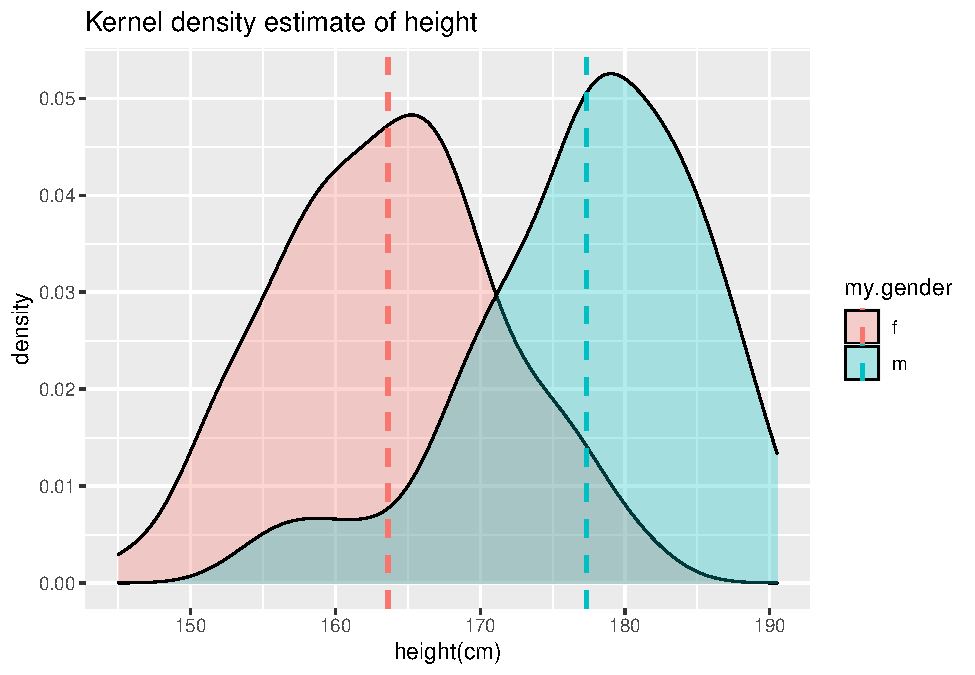
\includegraphics[trim = 0 0 0 0,clip,width=0.65\textwidth]{pdfs/kernel_density-1.pdf} }
    \end{center}
    \label{fig:height-dist}
    \hrule
\end{figure}

\noindent Figure \ref{fig:height-dist} visualizes the height
distributions of males and females in the sample data. The red line
indicates the mean value of the female height sample, and the blue line
indicates the mean value of the male height sample. The difference
between the average height is about 13.7cm, which is 1.3cm greater than
the global mean difference of 12cm, according to
\citep{owidhumanheight:2013}. In our sample data, men are about 8.4\%
taller than the female on average. The result verifies our sample data
is within the norm of global height difference.

\section{Research Question: Male and female comparison of body measurements and proportions }
\label{sec:rq}

\subsection{How are male and female differ in terms of body measurements}
\label{sec:rq2}

\begin{figure}[!ht]
    \hrule
    \caption{ \textbf{boxplots of male and female measurements} }
    \begin{center}
        \scalebox{1.00}{    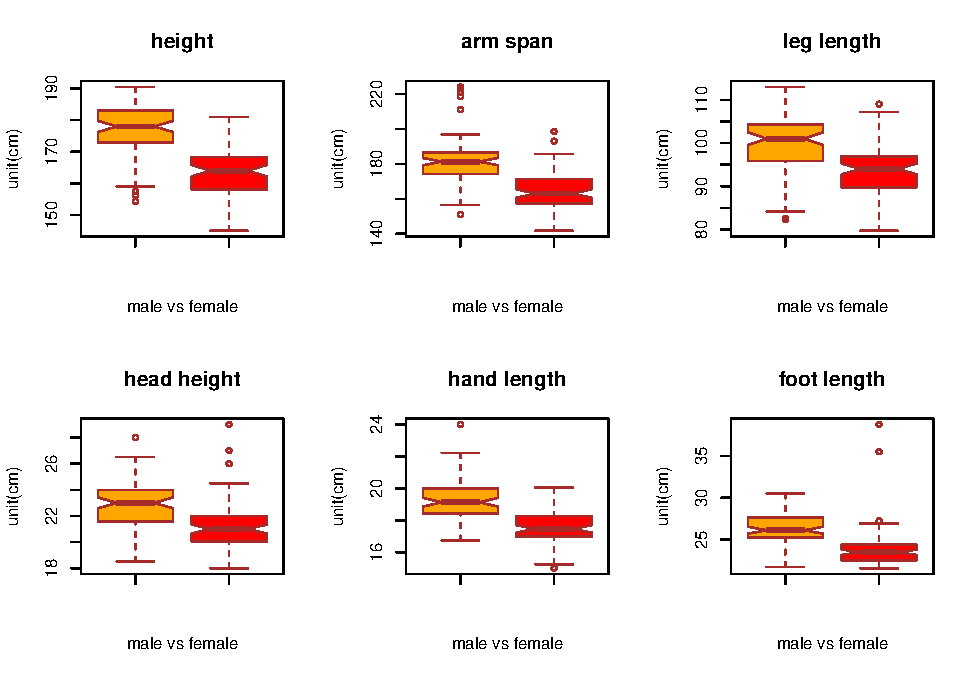
\includegraphics[trim = 0 0 0 0,clip,width=0.80\textwidth]{pdfs/measure_box_plots-1.pdf} }
    \end{center}
    \label{fig:measure.mf}
    \hrule
\end{figure}

\begin{figure}[!ht]
    \hrule
    \caption{ \textbf{boxplots of white/asian male and female body measurements} }
    \begin{center}
        \scalebox{1.00}{    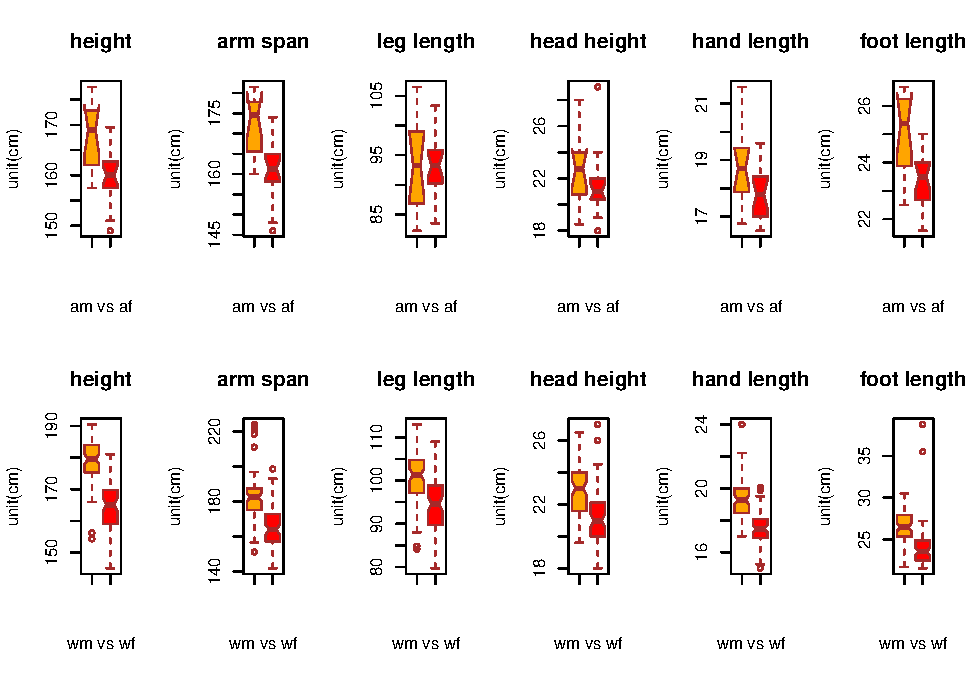
\includegraphics[trim = 0 0 0 0,clip,width=0.80\textwidth]{pdfs/measure_boxplot_amfwmf-1.pdf} }
    \end{center}
    \label{fig:measure.amfwmf}
    \hrule
\end{figure}

\noindent The sample data measurement differs between males and females.
Figure \ref{fig:measure.mf} reveal the distribution of each variable
between men and women. All variables median value lie outside of the box
of opposite sex box plots. That is, there is likely to be a difference
between the two genders. Observation of Interquartile ranges(the box)
shows a similar dispersion between males and females. The overall spread
of the boxplots reveals men vary more in head height and foot length in
comparison to women. Some of the outliers in head height, hand length,
and foot length are likely due to a measurement error. It is very
unlikely that the normal human head height and foot length exceed 30cm.
Extreme outliers will be removed for the hypothesis
testing.\vspace{0.25in}

\noindent Further investigating the measurement between male and female
with another factor variable ethnicity. In our sample, we are only
comparing Asians and whites. Figure \ref{fig:measure.amfwmf} displays
boxplots of Asian male and female measurements on the top row and white
male and female measurements on the bottom row. The boxplots are closer
together and overlap more in Asians than whites. This indicates there is
less difference between genders in Asians than whites. It is interesting
to observe leg length between Asian males and females, they seem to have
the same median value although Asian male's median height value is about
10cm taller. Do Asian women have longer leg lengths relative to height
than Asian men? Note the distribution of Asian males varies greater than
of Asian females across every measurement variables. The distribution of
white males and females is very similar to the average distribution
between males and females. However, the average measurement values in
whites are slightly higher than the average sample data.\vspace{0.25in}

\subsection{How are male and female differ in terms of body proportions}
\label{sec:rq3}

\begin{figure}[!ht]
    \hrule
    \caption{ \textbf{boxplots of male and female body proportions} }
    \begin{center}
        \scalebox{1.00}{    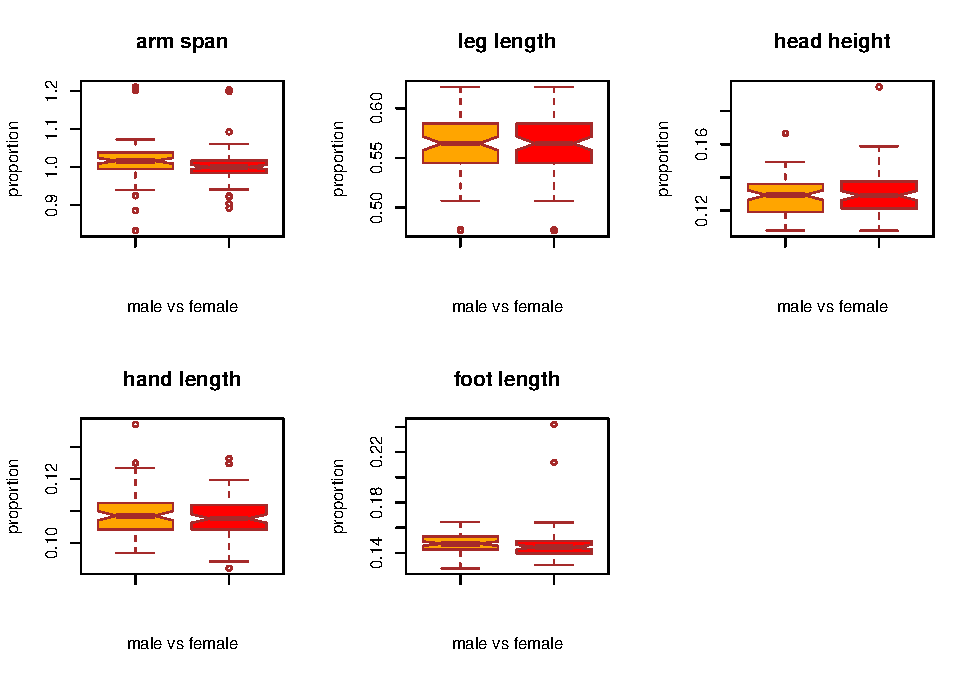
\includegraphics[trim = 0 0 0 0,clip,width=0.80\textwidth]{pdfs/proportion_box_plots-1.pdf} }
    \end{center}
    \label{fig:proportion.mf}
    \hrule
\end{figure}

\noindent In Figure \ref{fig:proportion.mf} The proportion of boxplots
between male and female sample data reveal the distribution of body
proportions relative to height. It is clear to see the distributions are
very similar to each other. Body proportion between males and females
doesn't seem to differ much. On average, the arm span is about the same
as the height of a person. The median head height proportion is about
0.13, which is about 7.7 heads will fit into a person's standing
height.\vspace{0.25in}

\begin{figure}[!ht]
    \hrule
    \caption{ \textbf{boxplots of white/asian male and female body proportions} }
    \begin{center}
        \scalebox{1.00}{    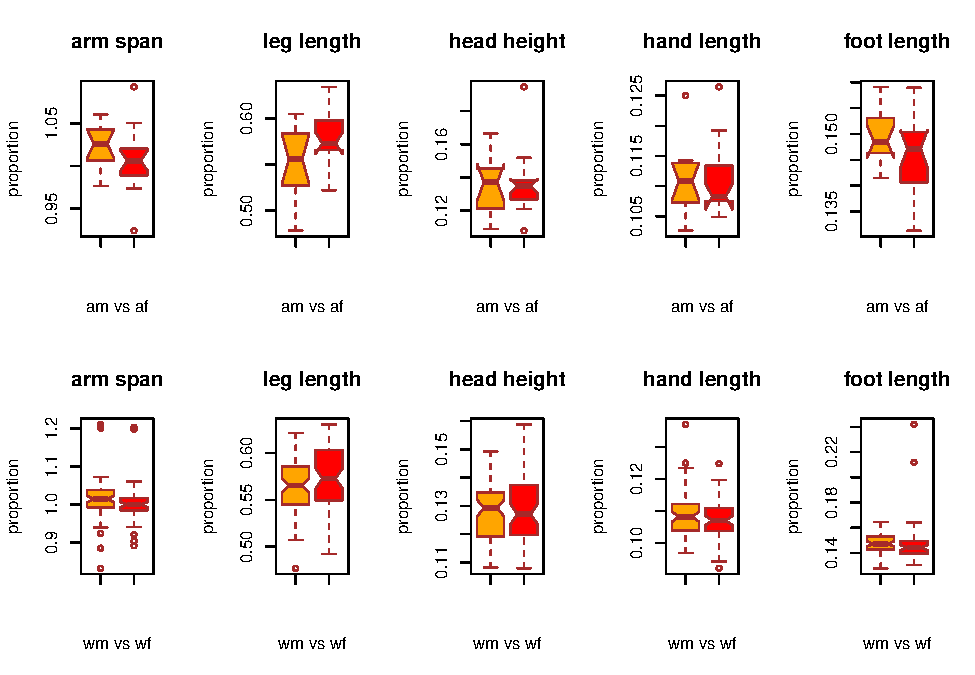
\includegraphics[trim = 0 0 0 0,clip,width=0.80\textwidth]{pdfs/proportion_box_plots_amfwmf-1.pdf} }
    \end{center}
    \label{fig:prportion.amfwmf}
    \hrule
\end{figure}

\noindent Figure \ref{fig:proportion.amfwmf} breaks down the male-female
proportion boxplots between Asian and white. Again, the boxplots overlap
with each other. However, the Asian male/female boxplots median values
differ slightly. Asian male boxplots show longer arm span and hand
length, and shorter leg length compared to Asian female proportions. In
the next section, the study reviews the significance of the difference
in body measurements and the proportion between genders.\vspace{0.25in}

\section{Data Description}
\label{sec:data}

\noindent Data was collected by each classmate. Each classmate created
handouts for data collection and collected 10 individuals measurements.
The original data initially contained 428 observations. After the data
cleaning process, the observation reduced to 190 individuals. Some of
the measurements measured right and left side of the body have been
merged into one averaged value. All the measurement units were converted
to centimeters.\vspace{0.25in}

\noindent Sample data constraints individuals at age 18 or above. The
measurements contain individuals' height, leg length, arm span, head
height, hand length, and foot length. The sample data also contains
proportions of each measurement relative to height. Other variables used
in the sample data include gender, sex, and age.\vspace{0.25in}

\noindent Reference the section in the Appendix with greater detail
about the data provenance \ref{sec:appendix}.

\subsection{Summary of Sample}
\label{sec:data-sample}

\noindent Figure\ref{fig:sample} shows the sample data counts grouped by
gender and ethnicity. A total of 167 observations are in sample data
which contains 83 females and 84 males. About 70\% of the sample data is
white and about 30\% Asian.

\begin{figure}[!ht]
    \hrule
    \caption{ \textbf{sample data grouping by gender and ethnicity} }
    \begin{center}
        \scalebox{1.00}{    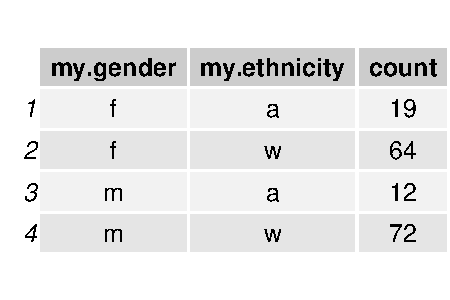
\includegraphics[trim = 0 0 0 0,clip,width=0.85\textwidth]{pdfs/sample.pdf} }
    \end{center}
    \label{fig:sample}
    \hrule
\end{figure}

\noindent Figure\ref{fig:age-dist} histogram shows the density of the
sample data in the different age groups. About 45\% of the participants
are aged between 20 and 30.

\begin{figure}[!ht]
    \hrule
    \caption{ \textbf{sample data age distribution} }
    \begin{center}
        \scalebox{1.00}{    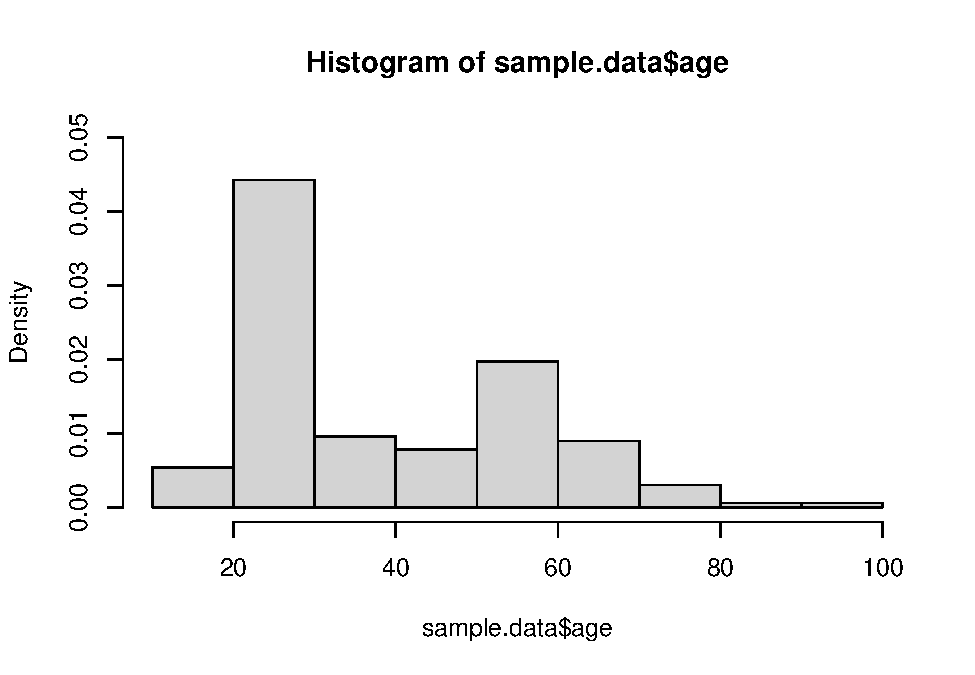
\includegraphics[trim = 0 0 0 0,clip,width=0.85\textwidth]{pdfs/sample_proportion-1.pdf} }
    \end{center}
    \label{fig:age-dist}
    \hrule
\end{figure}

\subsection{Summary Statistics of Data}
\label{sec:data-summary}

\noindent 

See table \ref{table:male-correlation} and
\ref{table:female-correlation} \newpage

% latex table generated in R 4.0.3 by xtable 1.8-4 package
% Mon Dec 14 22:41:11 2020
\begin{table}[ht]
\centering
\begin{tabular}{rrlrrrr}
  \hline
 & rank & title & year & ratings & votes & rank.popular \\ 
  \hline
&   1 & I Am Legend & 2007 & 7.20 & 675160 &  16 \\ 
&   2 & Suicide Squad & 2016 & 6.00 & 588064 &   4 \\ 
&   3 & Independence Day & 1996 & 7.00 & 520592 &  10 \\ 
&   4 & Men in Black & 1997 & 7.30 & 507597 &  19 \\ 
&   5 & I, Robot & 2004 & 7.10 & 491474 &  38 \\ 
&   6 & The Pursuit of Happyness & 2006 & 8.00 & 438121 &  27 \\ 
&   7 & Hancock & 2008 & 6.40 & 437887 &  39 \\ 
&   8 & Men in Black II & 2002 & 6.20 & 337458 &  36 \\ 
&   9 & Men in Black 3 & 2012 & 6.80 & 329948 &  48 \\ 
&  10 & Hitch & 2005 & 6.60 & 291991 &  35 \\ 
&  12 & Bad Boys & 1995 & 6.90 & 235766 &  12 \\ 
&  13 & Bad Boys II & 2003 & 6.60 & 228329 &  26 \\ 
&  14 & Enemy of the State & 1998 & 7.30 & 224019 &  32 \\ 
&  15 & Aladdin & 2019 & 7.00 & 216257 &  38 \\ 
&  16 & Austin Powers: The Spy Who Shagged Me & 1999 & 6.60 & 214064 &  27 \\ 
&  17 & Focus & 2015 & 6.60 & 212789 &  46 \\ 
&  23 & The Karate Kid & 2010 & 6.20 & 158842 &  10 \\ 
&  24 & Wild Wild West & 1999 & 5.00 & 151132 &  34 \\ 
&  25 & The Parent Trap & 1998 & 6.50 & 117780 &   8 \\ 
   \hline
\end{tabular}
\end{table}


\begin{table}[!htbp]
\footnotesize
\centering
\caption{\textbf{Descriptive Statistics and Correlation Analysis in female}}
\label{table:female-correlation}
\begin{tabularx}{0.8\textwidth}{{r@{ \ \ } p{15mm} r@{}lp{0.1mm} r@{}l p{0.5mm} r@{}l p{0.1mm} r@{}l p{0.1mm} r@{}l p{0.1mm} r@{}l p{0.1mm} r@{}l p{0.1mm}   r@{}l  }}
 & \\
\hline
 & \\
\multicolumn{2}{c}{\textbf{ }} & \multicolumn{2}{c}{\textbf{M}} & & \multicolumn{2}{c}{\textbf{SD}} &  & \multicolumn{2}{c}{\textbf{1}} &  & \multicolumn{2}{c}{\textbf{2}} &  & \multicolumn{2}{c}{\textbf{3}} &  & \multicolumn{2}{c}{\textbf{4}} &  & \multicolumn{2}{c}{\textbf{5}} &  & \\ 
 & \\
\hline
 & \\
\textbf{1} & \textbf{height} &  163&.6 &  &  7&.65 &  &  \multicolumn{2}{c}{1}  &  &  \multicolumn{2}{c}{ \  \  \  \  \ }  &  &  \multicolumn{2}{c}{ \  \  \  \  \ }  &  &  \multicolumn{2}{c}{ \  \  \  \  \ }  &  &  \multicolumn{2}{c}{ \  \  \  \  \ }  &  & \\ 
 & \\
\textbf{2} & \textbf{head.height} &  21&.3 &  &  1&.88 &  &  -&.05 &  &  \multicolumn{2}{c}{1}  &  &  \multicolumn{2}{c}{ \  \  \  \  \ }  &  &  \multicolumn{2}{c}{ \  \  \  \  \ }  &  &  \multicolumn{2}{c}{ \  \  \  \  \ }  &  & \\ 
 & \\
\textbf{3} & \textbf{arm.span} &  164&.2 &  &  10&.49 &  &  &.71{$^{***}$}  &  &  -&.15 &  &  \multicolumn{2}{c}{1}  &  &  \multicolumn{2}{c}{ \  \  \  \  \ }  &  &  \multicolumn{2}{c}{ \  \  \  \  \ }  &  & \\ 
 & \\
\textbf{4} & \textbf{hand.length} &  17&.6 &  &  1&.12 &  &  &.47{$^{***}$}  &  &  &.01 &  &  &.33{$^{**}$}  &  &  \multicolumn{2}{c}{1}  &  &  \multicolumn{2}{c}{ \  \  \  \  \ }  &  & \\ 
 & \\
\textbf{5} & \textbf{foot.length} &  23&.9 &  &  2&.51 &  &  &.33{$^{**}$}  &  &  &.04 &  &  &.32{$^{**}$}  &  &  &.38{$^{***}$}  &  &  \multicolumn{2}{c}{1}  &  & \\ 
 & \\
\textbf{6} & \textbf{floor.hip} &  94&.0 &  &  5&.47 &  &  &.49{$^{***}$}  &  &  &.05 &  &  &.38{$^{***}$}  &  &  &.41{$^{***}$}  &  &  &.31{$^{**}$}  &  & \\ 
 & \\
\hline
 & \\
\multicolumn{22}{p{0.72\textwidth}}{  \footnotesize { \begin{hangparas}{0.75in}{1} \textbf{\underline{Notes}:} \ \ Pearson pairwise correlations are reported; \newline a two-side test was performed to report correlation significance.  \end{hangparas} } }  & \\  
\multicolumn{22}{p{0.72\textwidth}}{  {\tiny {$^{\dagger} p < .10$} }  {     } {\tiny        {$^{*} p < .05$} }  {     } {\tiny       {$^{**} p < .01$} }  {     } {\tiny      {$^{***} p < .001$} } {     }     } & \\ 
 & \\
\hline
\end{tabularx}
\end{table}


\section{Key Findings}
\label{sec:findings}

\section{Conclusion}
\label{sec:conclusion}

\newpage

This was a new page

This is a newline. \newline  Here is some more text.

Below are some example code that may benefit you in preparing your
document. \newline

\vspace{0.25in}

\noindent Please state your name: \hrulefill \newline I was born on
\hrulefill in \hrulefill \vspace{0.25in}

\begin{equation}
\label{eq:my-model}
    Y_{jt} = \alpha + \bm{\beta}X_{jt} + \upsilon_{j}  + \varepsilon_{jt} ,
\end{equation}

\noindent where \(\alpha\) is the grand mean, \(\upsilon_{j}\) is the
fixed-time country mean, \(X_{jt}\) (country \(j\) at time \(t\)) is the
matrix of country-level observations for the vector of aforementioned
parameters \(\bm{\beta}\), and \(\varepsilon_{jt}\) represents the
residual idiosyncratic disturbance. Our panel data set consists of
repeated observations of countries over time. Therefore, we employ
cross-section time-series models. This approach redefines
Equation\textasciitilde{}\ref{eq:my-model} by subtracting time-demeaned
values. This \emph{within} transformation subtracts constant country
effects for the dependent variable \(\bar{Y_{j}}\), the predictor
variables \(\bar{X_{j}}\), and the intercept \(\bar{\upsilon_{j}}\):

\begin{equation}
\label{eq:my-random}
    (Y_{jt} - \theta \bar{Y_{j}}) = (1-\theta)\alpha + \bm{\beta}(X_{jt} - \bar{X_{j}}) +  (\upsilon_{jt} - \theta \bar{\upsilon_{j}})  ,
\end{equation}

\noindent If \(\theta = 0\), the model reduces to a basic pooled
ordinary-least-squares (OLS) model; if \(\theta = 1\), the model reduces
to a fixed-effects model; otherwise the model represents a
random-effects model. The pooled OLS estimation is biased if country
effects exist \citep{Hsiao:2003}. The random-effects model may be
susceptible to omitted-variable bias \citep{Wooldridge:2006}: bias
because a predictor was excluded from the model specification.
Conversely, the fixed-effects model is not susceptible to this bias as
it captures unobserved intracountry variation around its average
country-level ``fixed effect." Panel-data analysis commonly has issues
with heteroskedasticity, serial autocorrelation, and cross-sectional
autocorrelation.

\vspace{0.5in}

\(i=1\) and \[i = 1\]

\vspace{0.5in}

\begin{tabular}{ c c c c c}
  1 & 2 & 3 & 4 & 5 \\
  \hline
  6 & 7 & 8 & 9 & 10
\end{tabular}

\vspace{0.5in}

\begin{figure}[!ht]
%% figures have hrule, tables have hline
    \hrule
    \caption{ \textbf{Conceptual Model} }
    \begin{center}
        \scalebox{1.00}{    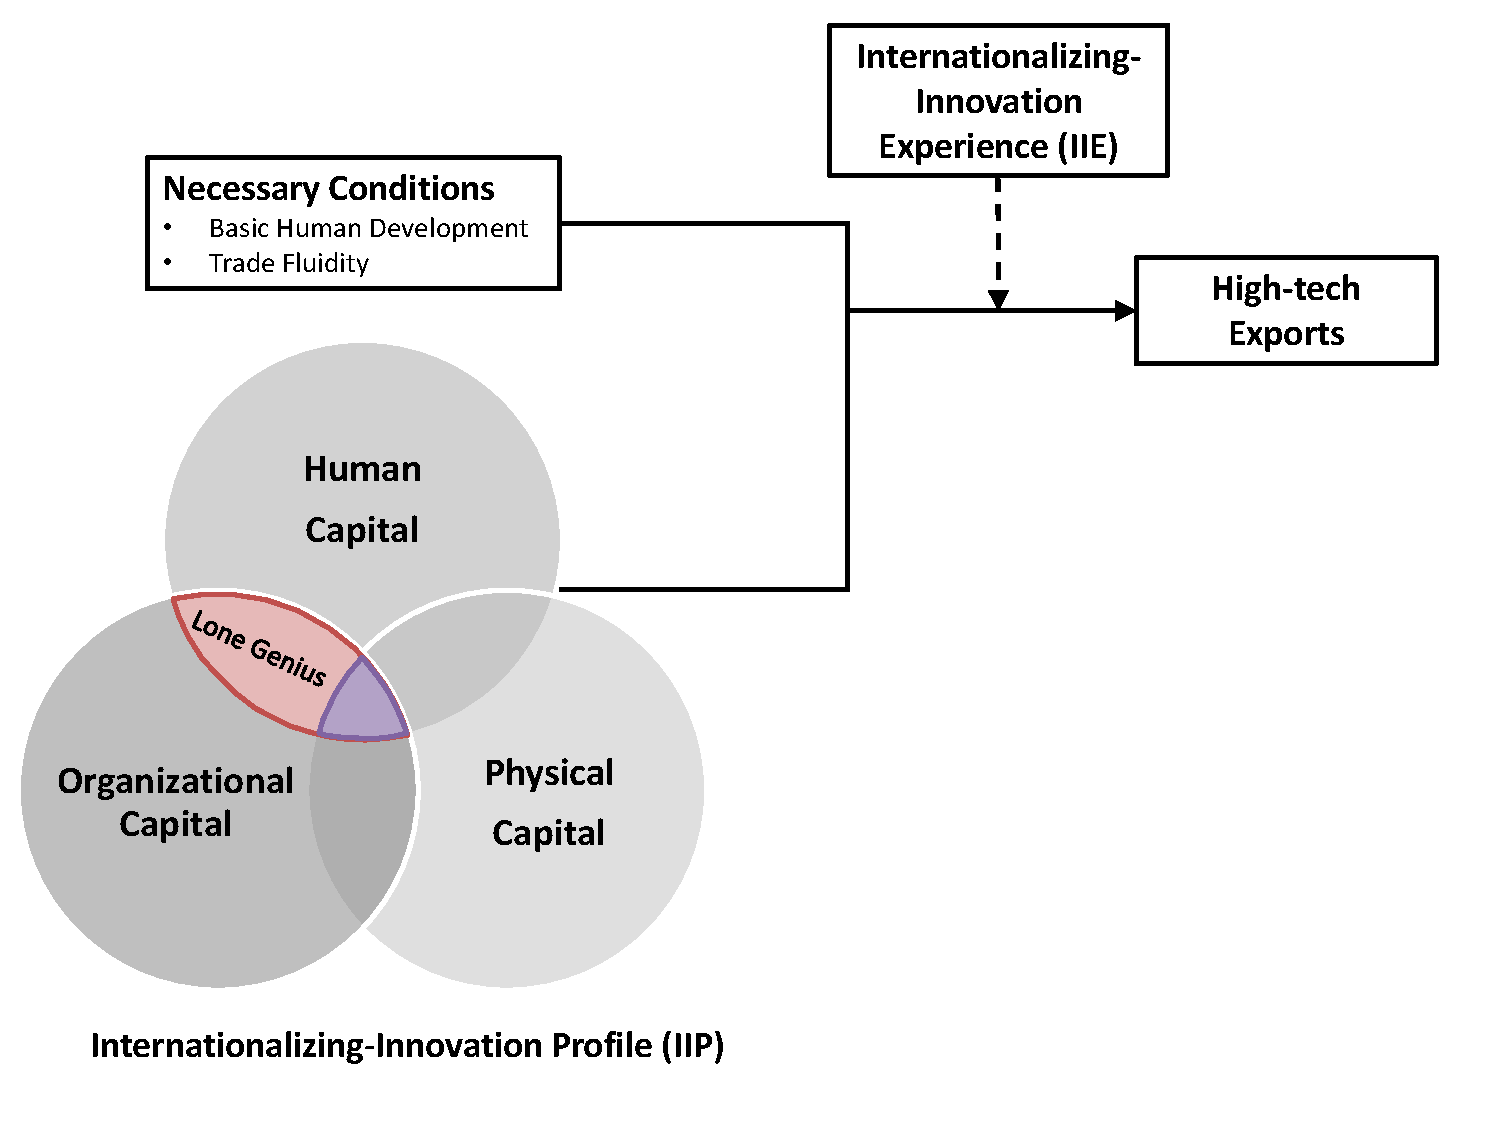
\includegraphics[trim = 0 0 0 0,clip,width=\textwidth]{figures/conceptual-model-v4.pdf} }
    \end{center}
    \label{fig:conceptual-model}
    \hrule
\end{figure}

See Figure \ref{fig:conceptual-model}.

\newpage

This is a
footnote\footnote{This is a footnote that can be really long.  \newline You can have multiple paragraphs in the footnote.  You can have \underline{underline} or \textbf{bold} or \emph{italics}.  You can even have a math equation inline. \newline In this section, we review the regression results to summarize our findings.  First, we examine each model for significance, and conclude the hypothesized models fit well with the data.  Second, we conclude that the fixed country effects represent consistent and unbiased parameter estimates.  Third, with the use of the \citet{Driscoll:1998} robust standard errors, we adjust any variance bias to ascertain the significance of these consistent estimates.  Therefore, we are able to make inferences about the hypotheses using our model estimates.  For ease of interpretation across these 12 models, we introduce $\betaSH{{ \ \ }M1}{Total}{1}$ as notation to refer to parameter estimate $\hat{\beta}_{1}$ (HDI) for the Total Sample and (M1) Model 1:  Main Effects.  We proceed by reporting findings for the total sample. \newline The footnotes are automatically converted to "endnotes" and will be included at the end of the document.  It will finish when you have that outer brace like this.}
that can be placed within a document.

\vspace{1.5in}

Refer to the Appendices in section\textasciitilde{}\ref{sec:appendix}
where I am going to cite John \citep[pp. 2-3]{Tukey:1962}.

Here is a quote by \citet[pp. 2-3]{Tukey:1962}:

\begin{quote}
For a long time I have thought I was a statistician, interested in inferences from the particular to the general.  But as I have watched mathematical statistics evolve, I have had to cause to wonder and to doubt. [...] All in all, I have come to feel that my central interest is in \emph{data analysis}, which I take to include among other things: procedures for analyzing data, techniques for interpreting the results of such procedures, ways of planning the gathering of data to make its analysis easier, more precise or more accurate, and all the machinery and results of (mathematical) statistics which apply to analyzing the data.

Large parts of data analysis are inferential in the sample-to-population sense, but these are only parts, not the whole.  Large parts of data analysis are incisive, laying bare indications which we could not perceive by simple and direct examination of the raw data, but these too are only parts, not the whole.  Some parts of data analysis, as the term is her stretch beyond its philology, are allocation, in the sense that they guide us in the distribution of effort and other valuable considerations in observation, experimentation, or analysis.  Data analysis is a larger and more varied field than inference, or incisive procedures, or allocation.

Statistics has contributed much to data analysis.  In the future it can, and in my view should, contribute more.  For such contributions to exist, and be valuable, it is not necessary that they be direct.  They need not provide new techniques, or better tables for old techniques, in order to influence the practice of data analysis.
\end{quote}

\newpage
\section{APPENDICES}
\label{sec:appendix}

\subsection{Data Provenance}
\label{sec:appendix-data-provenance}

\newpage
\subsubsection{Data Collection Handout}
\label{sec:appendix-data-handout}

\begin{figure}[!ht]
    \hrule
    \caption{ \textbf{Handout Page 1} }
    \begin{center}
        \scalebox{1.00}{    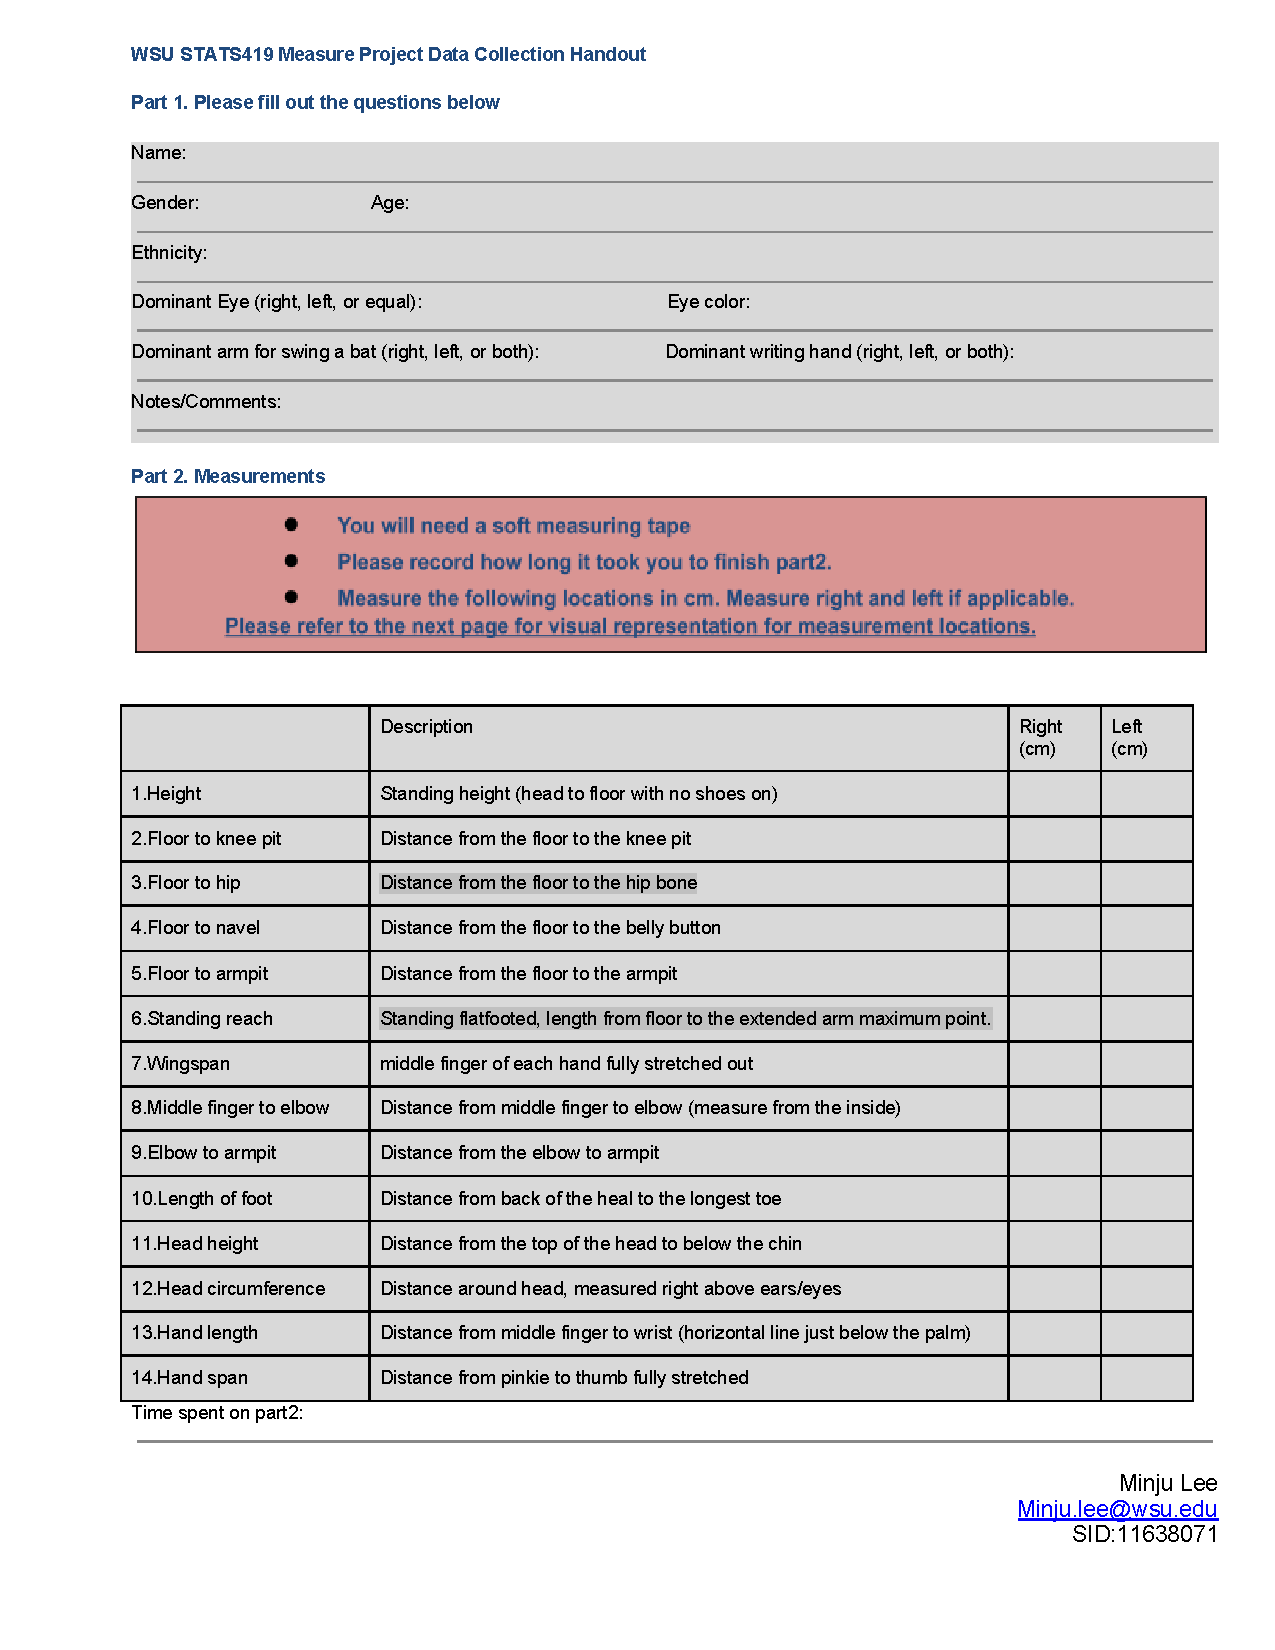
\includegraphics[trim = 0 0 0 0,clip,width=0.85\textwidth]{pdfs/handout1.pdf} }
    \end{center}
    \label{fig:handout-1}
    \hrule
\end{figure}

\newpage

\begin{figure}[!ht]
    \hrule
    \caption{ \textbf{Handout Page 2} }
    \begin{center}
        \scalebox{1.00}{    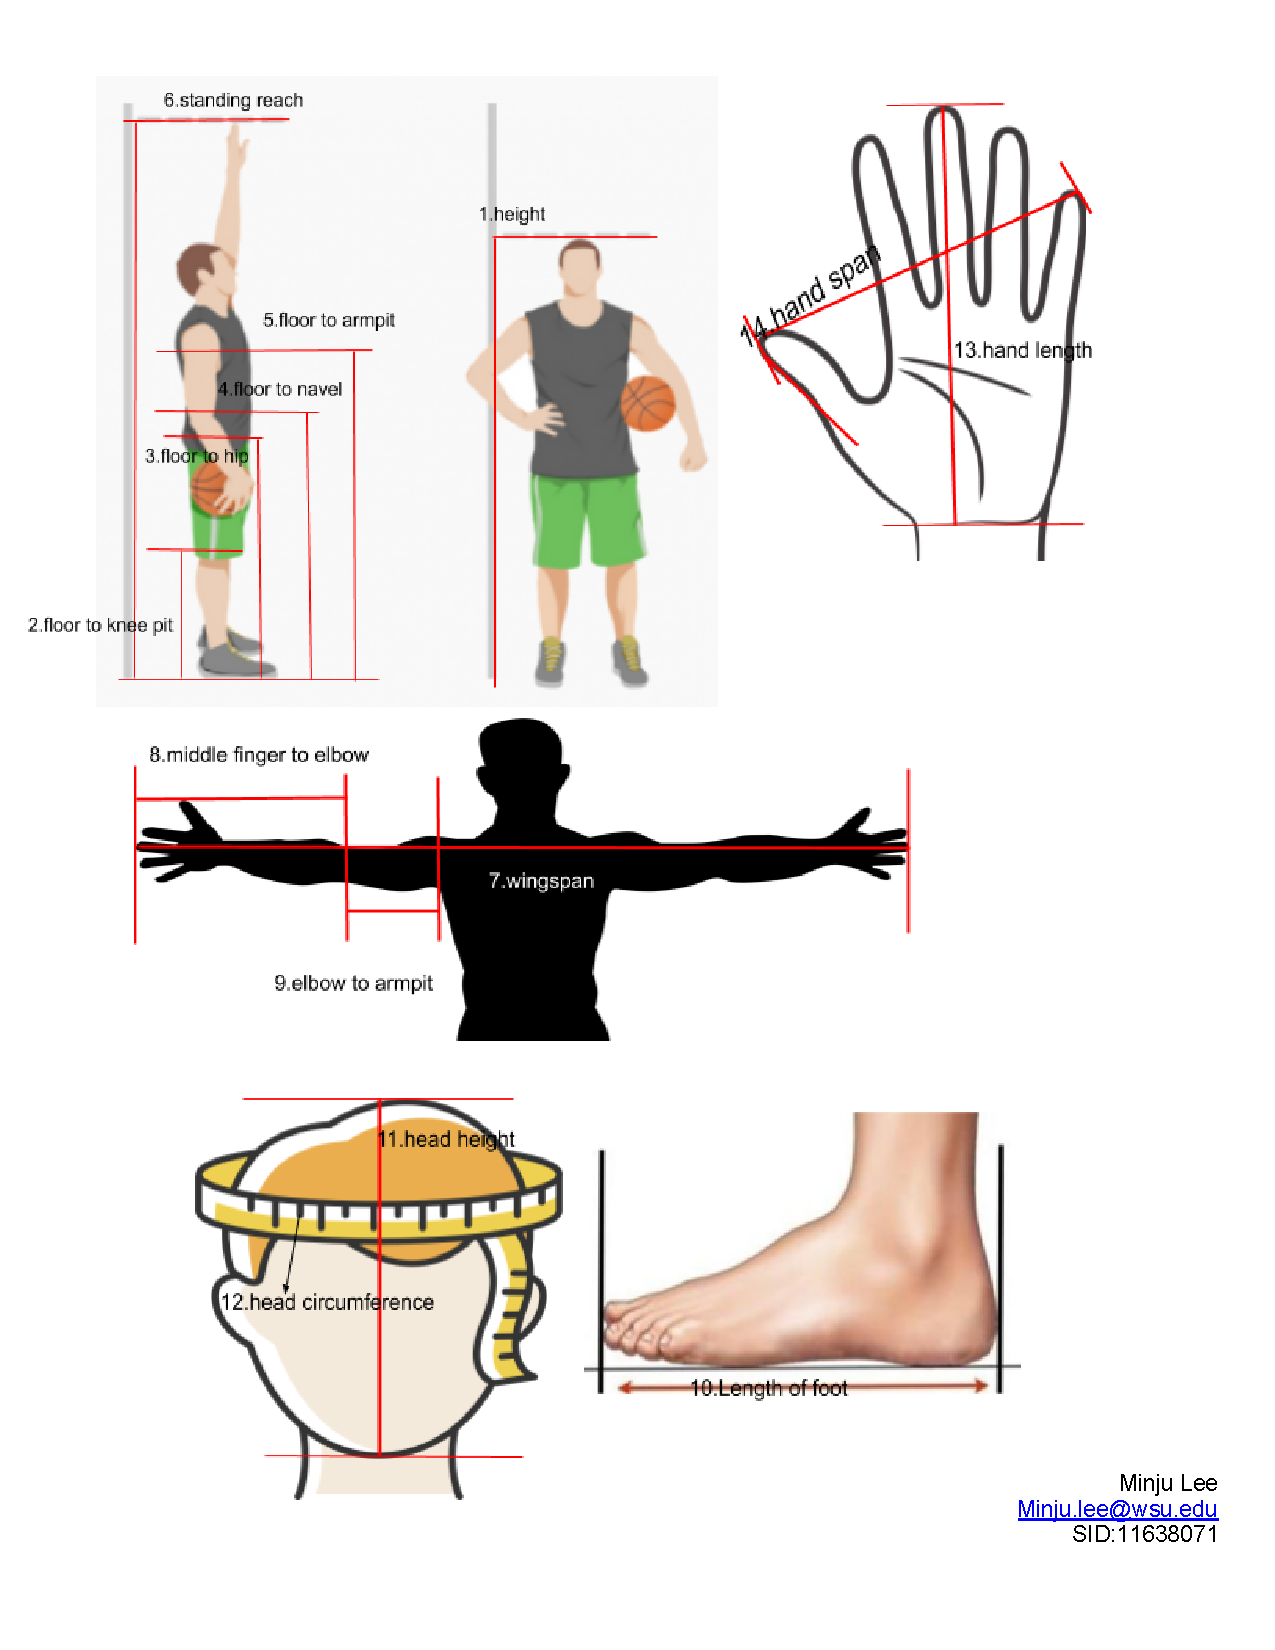
\includegraphics[trim = 0 0 0 0,clip,width=0.85\textwidth]{pdfs/handout2.pdf} }
    \end{center}
    \label{fig:handout-2}
    \hrule
\end{figure}

\newpage

\begin{figure}[!ht]
    \begin{subfigure}[h]{0.5\textwidth}
    \centering
    %  trim={<left> <lower> <right> <upper>}
    % https://shantoroy.com/latex/add-subfig-in-latex/
            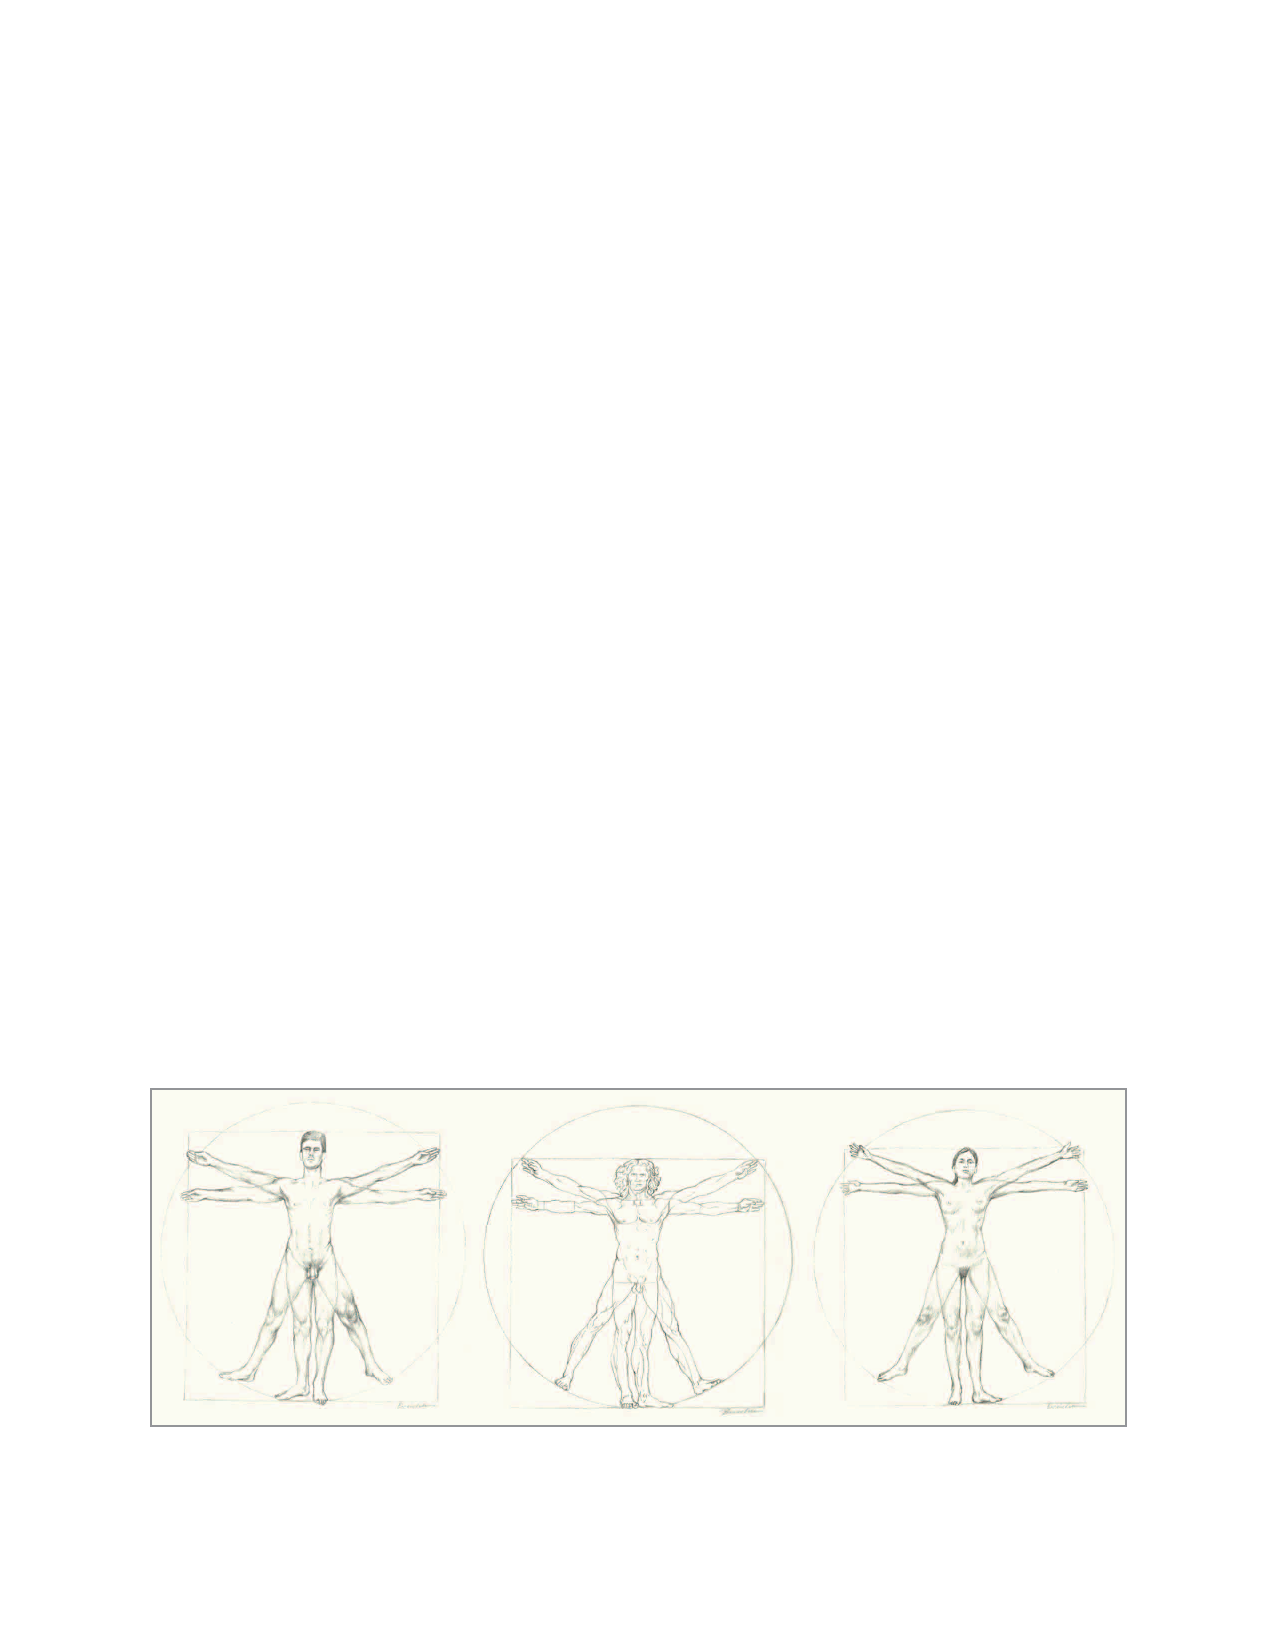
\includegraphics[trim = 0 0 11.25cm 0,clip,scale=1]{figures/Vitruvian.pdf}
        \caption{ \citet{Thomas:2020} discuss this. }
        \label{fig:sub-first}
    \end{subfigure}
    \begin{subfigure}[h]{0.5\textwidth}
    \centering
        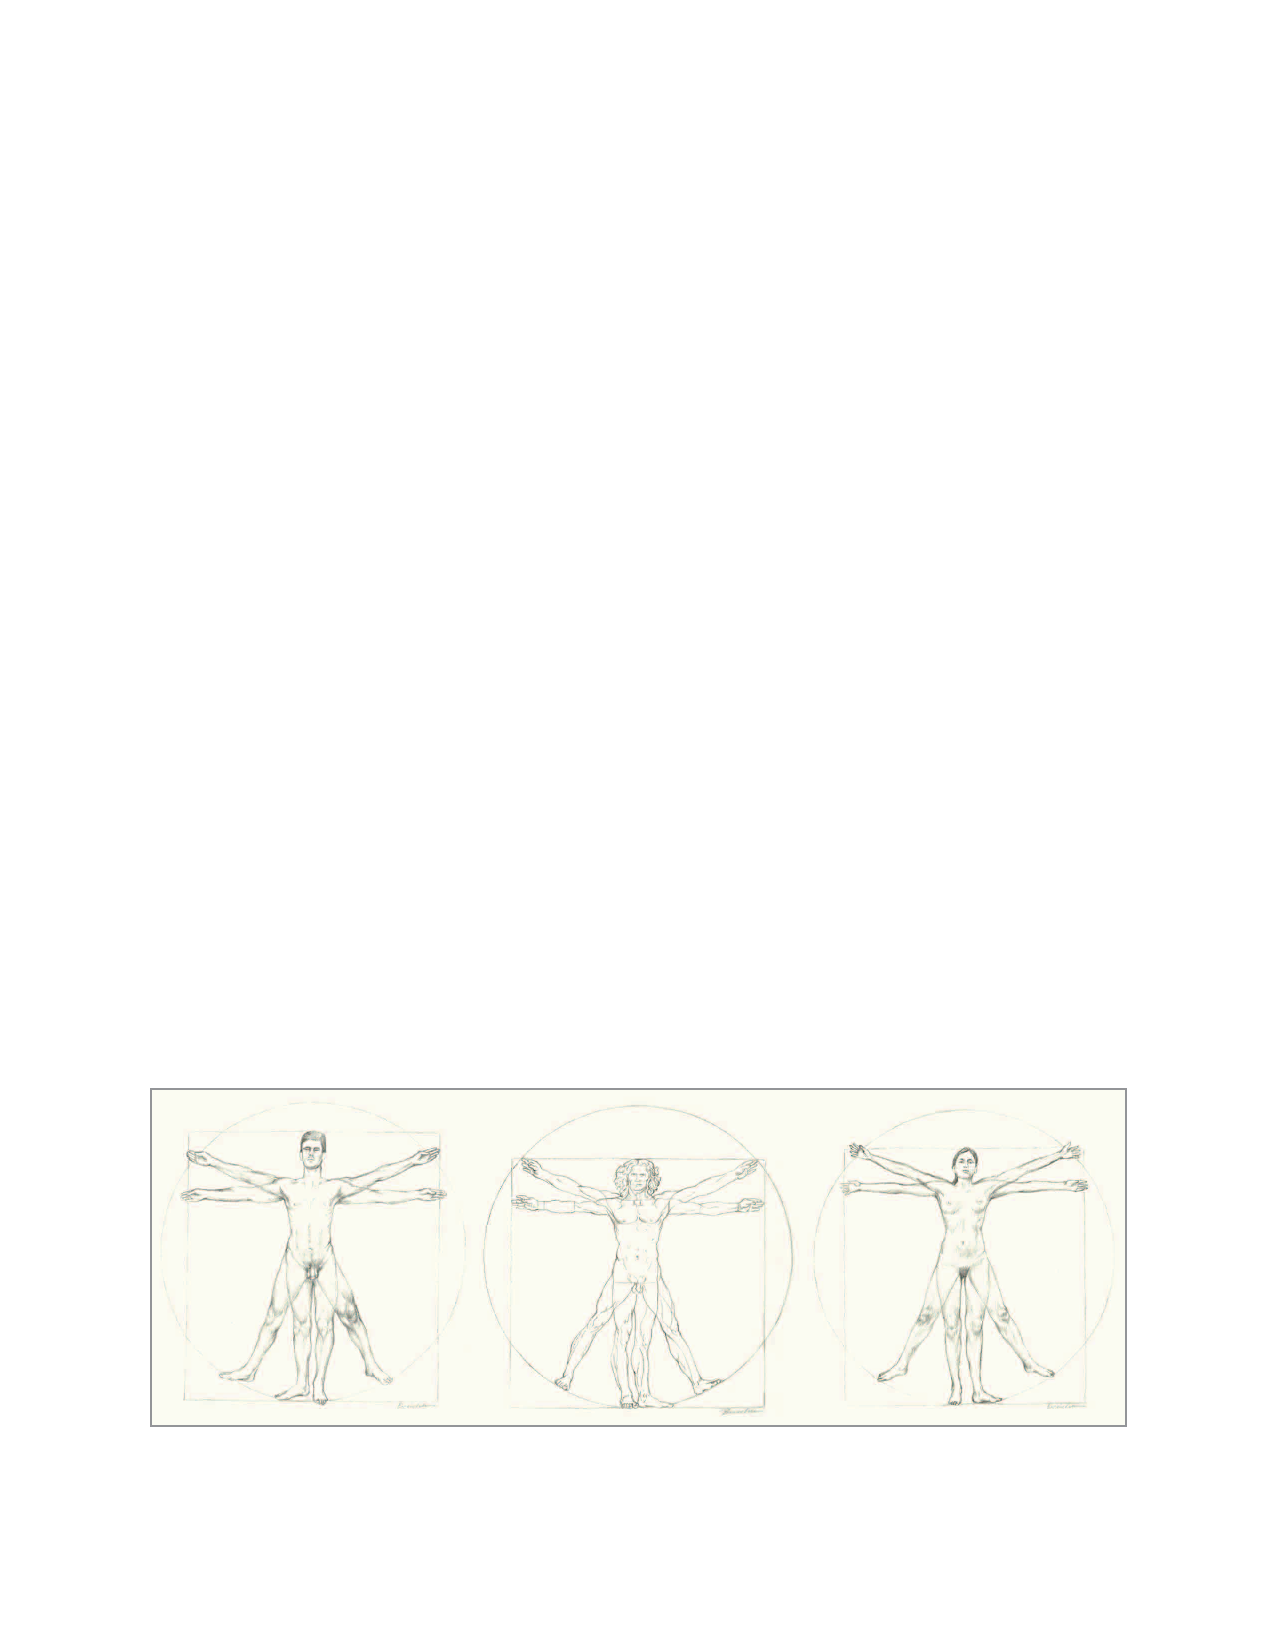
\includegraphics[trim = 11.25cm 0 0 0,clip,scale=1]{figures/Vitruvian.pdf}
            \caption{Schnitt realer Sensor \citep{Thomas:2020}}
        \label{fig:sub-second}
    \end{subfigure}
    \vspace{2.5mm}
    \hrule
    \vspace{2.5mm}
        \caption{\textbf{ Der Sensor in Theorie und Verwirklichung... caption at bottom instead? }  I can write a really long caption if I want. \newline This is using "crop" to include one image and trim it to appear as two.  Likely you will have two separate images if you use this option, so you would set the trim parameters all equal to 0.  \newline   This figure has subfigures which each also have a possible caption.   }
        \label{fig:combined}
    \vspace{-2.5mm}
    \hrule
\end{figure}

\newpage

\subsection{Preparing the Report Workspace as a subsection}
\label{sec:appendix-setup}

\subsubsection{prepare sample data}
\label{sec:appendix-setup2}

Below is the necessary functions and libraries required to run the code
referenced in this document.

\begin{Shaded}
\begin{Highlighting}[]
\KeywordTok{library}\NormalTok{(devtools);       }\CommentTok{\# required for source\_url}
\end{Highlighting}
\end{Shaded}

\begin{verbatim}
## Loading required package: usethis
\end{verbatim}

\begin{Shaded}
\begin{Highlighting}[]
\NormalTok{path.humanVerseWSU =}\StringTok{ "https://raw.githubusercontent.com/MonteShaffer/humanVerseWSU/"}
\KeywordTok{source\_url}\NormalTok{( }\KeywordTok{paste0}\NormalTok{(path.humanVerseWSU,}\StringTok{"master/misc/functions{-}project{-}measure.R"}\NormalTok{) );}
\end{Highlighting}
\end{Shaded}

\begin{verbatim}
## SHA-1 hash of file is 091aa1c443f262dce181395047d037a756331a65
\end{verbatim}

\begin{verbatim}
## Loading required package: lattice
\end{verbatim}

\begin{verbatim}
## Loading required package: survival
\end{verbatim}

\begin{verbatim}
## Loading required package: Formula
\end{verbatim}

\begin{verbatim}
## Loading required package: ggplot2
\end{verbatim}

\begin{verbatim}
## 
## Attaching package: 'Hmisc'
\end{verbatim}

\begin{verbatim}
## The following objects are masked from 'package:base':
## 
##     format.pval, units
\end{verbatim}

\begin{Shaded}
\begin{Highlighting}[]
\KeywordTok{source\_url}\NormalTok{( }\KeywordTok{paste0}\NormalTok{(path.humanVerseWSU,}\StringTok{"master/humanVerseWSU/R/functions{-}dataframe.R"}\NormalTok{) );}
\end{Highlighting}
\end{Shaded}

\begin{verbatim}
## SHA-1 hash of file is 1149cbf3e865f692b50d4d1983e6364dc56ce62d
\end{verbatim}

\begin{Shaded}
\begin{Highlighting}[]
\KeywordTok{source\_url}\NormalTok{( }\KeywordTok{paste0}\NormalTok{(path.humanVerseWSU,}\StringTok{"master/humanVerseWSU/R/functions{-}EDA.R"}\NormalTok{) );}
\end{Highlighting}
\end{Shaded}

\begin{verbatim}
## SHA-1 hash of file is 62ba3333da32792e57c410e3f02a443a4c7f4985
\end{verbatim}

\begin{verbatim}
## Welcome! Want to learn more? See two factoextra-related books at https://goo.gl/ve3WBa
\end{verbatim}

\begin{verbatim}
## 
## Attaching package: 'psych'
\end{verbatim}

\begin{verbatim}
## The following object is masked from 'package:Hmisc':
## 
##     describe
\end{verbatim}

\begin{verbatim}
## The following objects are masked from 'package:ggplot2':
## 
##     %+%, alpha
\end{verbatim}

Below is the code to load the data and prepare it for analysis.

\begin{Shaded}
\begin{Highlighting}[]
\NormalTok{path.project =}\StringTok{ "C:/\_git\_/WSU\_STATS419\_FALL2020/project{-}measure/"}\NormalTok{;}
\NormalTok{path.to.secret =}\StringTok{ "C:/Users/13608/Dropbox/WSU{-}419/Fall 2020/\_\_student\_access\_\_/\_SECRET\_/"}

\NormalTok{measure =}\StringTok{ }\NormalTok{utils}\OperatorTok{::}\KeywordTok{read.csv}\NormalTok{( }\KeywordTok{paste0}\NormalTok{(path.to.secret, }\StringTok{"measure{-}students.txt"}\NormalTok{), }\DataTypeTok{header=}\OtherTok{TRUE}\NormalTok{, }\DataTypeTok{quote=}\StringTok{""}\NormalTok{, }\DataTypeTok{sep=}\StringTok{"|"}\NormalTok{);}
\NormalTok{getOne =}\StringTok{ }\KeywordTok{c}\NormalTok{(}\StringTok{"hand.length"}\NormalTok{, }\StringTok{"hand.width"}\NormalTok{, }\StringTok{"hand.elbow"}\NormalTok{, }\StringTok{"elbow.armpit"}\NormalTok{, }\StringTok{"arm.reach"}\NormalTok{, }\StringTok{"foot.length"}\NormalTok{, }\StringTok{"floor.kneepit"}\NormalTok{, }\StringTok{"floor.hip"}\NormalTok{, }\StringTok{"floor.armpit"}\NormalTok{);}

\CommentTok{\#\#\#\#\#\#\#\#\#\#\#\#\#\#\#\#\#\#\#\#\#\#\#\#\#\#\#\#\#\#\#\#\#\#\#\#\#\#\#\#\#\#\#\#\#\#\#\#\#\#\#\#\#\#\#\#\#\#\#\#\#\#\#\#\#\#\#\#\#\#\#\#\#\#\#\#\#\#\#\#\#\#\#\#\#\#\#\#\#\#\#\#\#\#\#}
\NormalTok{path.github =}\StringTok{ "https://raw.githubusercontent.com/minju{-}lee92/WSU\_STATS419\_FALL2020/"}\NormalTok{;}
\KeywordTok{source\_url}\NormalTok{( }\KeywordTok{paste0}\NormalTok{(path.github,}\StringTok{"master/functions/functions{-}project{-}measure.R"}\NormalTok{) );}
\end{Highlighting}
\end{Shaded}

\begin{verbatim}
## SHA-1 hash of file is 5aa82ee87a0a62bfc9b04ccc942d44c0cc3ed092
\end{verbatim}

\begin{Shaded}
\begin{Highlighting}[]
\CommentTok{\# this is your function}
\CommentTok{\# covert unit into cm}
\NormalTok{measureAscm \textless{}{-}}\KeywordTok{convert.inchestocm}\NormalTok{(measure)}
\CommentTok{\# build merged left/right value cols}
\NormalTok{merged.df \textless{}{-}}\KeywordTok{merge.left.right}\NormalTok{(measureAscm, getOne)}
\CommentTok{\# remove nas, duplicates, create categorical variables... etc }
\NormalTok{cleaned.df =}\StringTok{ }\KeywordTok{prepareMeasureData}\NormalTok{(merged.df)}

\CommentTok{\# create scaled variables using height}
\NormalTok{colnum =}\StringTok{ }\KeywordTok{c}\NormalTok{(}\DecValTok{3}\OperatorTok{:}\DecValTok{7}\NormalTok{,}\DecValTok{20}\OperatorTok{:}\DecValTok{28}\NormalTok{)}
\NormalTok{new.colname =}\StringTok{ }\KeywordTok{c}\NormalTok{(}\StringTok{"p.height"}\NormalTok{, }\StringTok{"p.head.h"}\NormalTok{, }\StringTok{"p.head.c"}\NormalTok{, }\StringTok{"p.arm.span"}\NormalTok{, }\StringTok{"p.floor.navel"}\NormalTok{,}\StringTok{"p.hand.length"}\NormalTok{,}\StringTok{"p.hand.width"}\NormalTok{,}\StringTok{"p.hand.elbow"}\NormalTok{,}\StringTok{"p.elbow.armpit"}\NormalTok{,}\StringTok{"p.arm.reach"}\NormalTok{,}\StringTok{"p.foot.length"}\NormalTok{,}\StringTok{"p.floor.kneepit"}\NormalTok{, }\StringTok{"p.floor.hip"}\NormalTok{, }\StringTok{"p.floor.armpit"}\NormalTok{)}

\NormalTok{v1.df =}\KeywordTok{build.scale.variables}\NormalTok{(cleaned.df, colnum, new.colname, cleaned.df}\OperatorTok{$}\NormalTok{height)}

\CommentTok{\# final sample data for the analysis}
\NormalTok{sample.df \textless{}{-}v1.df[,}\KeywordTok{c}\NormalTok{(}\DecValTok{1}\OperatorTok{:}\DecValTok{4}\NormalTok{,}\DecValTok{6}\NormalTok{,}\DecValTok{20}\NormalTok{,}\DecValTok{25}\NormalTok{,}\DecValTok{27}\NormalTok{,}\DecValTok{13}\NormalTok{,}\DecValTok{29}\OperatorTok{:}\DecValTok{31}\NormalTok{,}\DecValTok{36}\NormalTok{,}\DecValTok{37}\NormalTok{,}\DecValTok{39}\NormalTok{,}\DecValTok{41}\NormalTok{,}\DecValTok{46}\NormalTok{,}\DecValTok{48}\NormalTok{)]}
\NormalTok{sample.data \textless{}{-}}\StringTok{ }\NormalTok{sample.df[sample.df}\OperatorTok{$}\NormalTok{my.gender }\OperatorTok{!=}\StringTok{\textquotesingle{}o\textquotesingle{}}\OperatorTok{\&}\StringTok{ }\NormalTok{sample.df}\OperatorTok{$}\NormalTok{my.ethnicity}\OperatorTok{==}\StringTok{\textquotesingle{}a\textquotesingle{}}\OperatorTok{|}\NormalTok{sample.df}\OperatorTok{$}\NormalTok{my.ethnicity}\OperatorTok{==}\StringTok{\textquotesingle{}w\textquotesingle{}}\NormalTok{,]}

\CommentTok{\# age over 18}
\NormalTok{sample.data \textless{}{-}}\StringTok{ }\NormalTok{sample.data[sample.data}\OperatorTok{$}\NormalTok{age }\OperatorTok{\textgreater{}=}\DecValTok{18}\NormalTok{,]}
\KeywordTok{summary}\NormalTok{(sample.data)}
\CommentTok{\# getting rid of outliers.}
\NormalTok{sample.data \textless{}{-}}\StringTok{ }\NormalTok{sample.data[sample.data}\OperatorTok{$}\NormalTok{height }\OperatorTok{\textgreater{}=}\StringTok{ }\DecValTok{145} \OperatorTok{\&}\StringTok{ }\NormalTok{sample.data}\OperatorTok{$}\NormalTok{arm.span}\OperatorTok{\textgreater{}}\DecValTok{100} \OperatorTok{\&}\StringTok{ }\NormalTok{sample.data}\OperatorTok{$}\NormalTok{hand.length}\OperatorTok{\textgreater{}}\DecValTok{10} \OperatorTok{\&}\StringTok{ }\NormalTok{sample.data}\OperatorTok{$}\NormalTok{hand.length}\OperatorTok{\textless{}}\DecValTok{30} \OperatorTok{\&}\StringTok{ }\NormalTok{sample.data}\OperatorTok{$}\NormalTok{foot.length}\OperatorTok{\textgreater{}}\DecValTok{19} \OperatorTok{\&}\StringTok{ }\NormalTok{sample.data}\OperatorTok{$}\NormalTok{floor.hip}\OperatorTok{\textgreater{}}\DecValTok{50} \OperatorTok{\&}\StringTok{ }\NormalTok{sample.data}\OperatorTok{$}\NormalTok{head.height}\OperatorTok{\textless{}}\DecValTok{30}\NormalTok{,]}

\KeywordTok{saveRDS}\NormalTok{(sample.data,}\StringTok{"sample.data.rds"}\NormalTok{);}
\NormalTok{    utils}\OperatorTok{::}\KeywordTok{write.table}\NormalTok{(sample.data, }\DataTypeTok{file=}\StringTok{"sample.data.txt"}\NormalTok{, }\DataTypeTok{quote=}\OtherTok{FALSE}\NormalTok{, }\DataTypeTok{col.names=}\OtherTok{TRUE}\NormalTok{, }\DataTypeTok{row.names=}\OtherTok{FALSE}\NormalTok{, }\DataTypeTok{sep=}\StringTok{"|"}\NormalTok{);}
\end{Highlighting}
\end{Shaded}

\subsubsection{generate summary of sample}
\label{sec:appendix-setup2}

\begin{Shaded}
\begin{Highlighting}[]
\KeywordTok{library}\NormalTok{(dplyr)}
\end{Highlighting}
\end{Shaded}

\begin{verbatim}
## 
## Attaching package: 'dplyr'
\end{verbatim}

\begin{verbatim}
## The following objects are masked from 'package:Hmisc':
## 
##     src, summarize
\end{verbatim}

\begin{verbatim}
## The following objects are masked from 'package:stats':
## 
##     filter, lag
\end{verbatim}

\begin{verbatim}
## The following objects are masked from 'package:base':
## 
##     intersect, setdiff, setequal, union
\end{verbatim}

\begin{Shaded}
\begin{Highlighting}[]
\NormalTok{sample.data \textless{}{-}}\StringTok{ }\KeywordTok{na.omit}\NormalTok{(sample.data)}
\NormalTok{dist.sample \textless{}{-}}\StringTok{ }\NormalTok{sample.data }\OperatorTok{\%\textgreater{}\%}\StringTok{ }\KeywordTok{group\_by}\NormalTok{(my.gender, my.ethnicity) }\OperatorTok{\%\textgreater{}\%}\StringTok{ }\NormalTok{dplyr}\OperatorTok{::}\KeywordTok{summarise}\NormalTok{(}\DataTypeTok{count =} \KeywordTok{n}\NormalTok{())}
\end{Highlighting}
\end{Shaded}

\begin{verbatim}
## `summarise()` regrouping output by 'my.gender' (override with `.groups` argument)
\end{verbatim}

\begin{Shaded}
\begin{Highlighting}[]
\KeywordTok{library}\NormalTok{(gridExtra)}
\end{Highlighting}
\end{Shaded}

\begin{verbatim}
## 
## Attaching package: 'gridExtra'
\end{verbatim}

\begin{verbatim}
## The following object is masked from 'package:dplyr':
## 
##     combine
\end{verbatim}

\begin{Shaded}
\begin{Highlighting}[]
\KeywordTok{pdf}\NormalTok{(}\StringTok{"pdfs/sample.pdf"}\NormalTok{, }\DataTypeTok{height=}\DecValTok{2}\NormalTok{, }\DataTypeTok{width=}\DecValTok{3}\NormalTok{)}
\KeywordTok{grid.table}\NormalTok{(dist.sample)}
\KeywordTok{dev.off}\NormalTok{()}


\KeywordTok{hist}\NormalTok{(sample.data}\OperatorTok{$}\NormalTok{age, }\DataTypeTok{breaks=}\KeywordTok{seq}\NormalTok{(}\DecValTok{10}\NormalTok{,}\DecValTok{100}\NormalTok{,}\DecValTok{10}\NormalTok{), }\DataTypeTok{ylim=}\KeywordTok{c}\NormalTok{(}\DecValTok{0}\NormalTok{,}\FloatTok{0.05}\NormalTok{), }\DataTypeTok{freq=}\OtherTok{FALSE}\NormalTok{)}
\end{Highlighting}
\end{Shaded}

\begin{Shaded}
\begin{Highlighting}[]
\KeywordTok{dim}\NormalTok{(sample.data)}
\KeywordTok{str}\NormalTok{(sample.data)}
\NormalTok{summary.sample \textless{}{-}}\KeywordTok{summary}\NormalTok{(sample.data[,}\KeywordTok{c}\NormalTok{(}\DecValTok{13}\OperatorTok{:}\DecValTok{18}\NormalTok{)])}
\KeywordTok{library}\NormalTok{(gridExtra)}
\KeywordTok{pdf}\NormalTok{(}\StringTok{"pdfs/summary{-}sample.pdf"}\NormalTok{, }\DataTypeTok{height=}\DecValTok{3}\NormalTok{, }\DataTypeTok{width=}\DecValTok{10}\NormalTok{)}
\KeywordTok{grid.table}\NormalTok{(summary.sample)}
\KeywordTok{dev.off}\NormalTok{()}
\end{Highlighting}
\end{Shaded}

\subsubsection{generate summary statistic tables}
\label{sec:appendix-setup2}

Below is the code to generate the summary statistics and save them as a
table that you see in Section \ref{table:correlation}.

\begin{Shaded}
\begin{Highlighting}[]
\NormalTok{path.project =}\StringTok{ "C:/\_git\_/WSU\_STATS419\_FALL2020/project{-}measure/"}\NormalTok{;}
\NormalTok{path.tables =}\StringTok{ }\KeywordTok{paste0}\NormalTok{(path.project,}\StringTok{"tables/"}\NormalTok{);}
  \KeywordTok{createDirRecursive}\NormalTok{(path.tables);}
\end{Highlighting}
\end{Shaded}

\begin{Shaded}
\begin{Highlighting}[]
\NormalTok{file.correlation =}\StringTok{ }\KeywordTok{paste0}\NormalTok{(path.tables,}\StringTok{"correlation{-}table.tex"}\NormalTok{)}
\NormalTok{myData =}\StringTok{ }\KeywordTok{as.matrix}\NormalTok{(sample.data[,}\KeywordTok{c}\NormalTok{(}\DecValTok{3}\OperatorTok{:}\DecValTok{8}\NormalTok{)])  }\CommentTok{\# numeric values only, only what will appear in table}
\CommentTok{\# https://www.overleaf.com/read/srzhrcryjpwn}
\CommentTok{\# keepaspectratio of include graphics }
\CommentTok{\# could scale \textbackslash{}input if still too big ...}
\CommentTok{\# https://tex.stackexchange.com/questions/13460/scalebox{-}knowing{-}how{-}much{-}it{-}scales\#13487}
\KeywordTok{buildLatexCorrelationTable}\NormalTok{(myData, }
  \DataTypeTok{rotateTable =} \OtherTok{FALSE}\NormalTok{,}
  \DataTypeTok{width.table =} \FloatTok{0.80}\NormalTok{, }\CommentTok{\# best for given data ... 0.95 when rotateTable = FALSE}
                      \CommentTok{\# 0.60 when rotateTable = TRUE}
  \DataTypeTok{myCaption =} \StringTok{"Overall Descriptive Statistics and Correlation Analysis"}\NormalTok{,}
  \DataTypeTok{myFile =}\NormalTok{ file.correlation,}
  \DataTypeTok{myNames =} \KeywordTok{colnames}\NormalTok{(myData),}
  \DataTypeTok{showOnes =} \StringTok{"left"}\NormalTok{)}
\KeywordTok{Sys.sleep}\NormalTok{(}\DecValTok{2}\NormalTok{) }\CommentTok{\# in case Knit{-}PDF doesn\textquotesingle{}t like that I just created the file...}
\end{Highlighting}
\end{Shaded}

\begin{Shaded}
\begin{Highlighting}[]
\NormalTok{file.correlation =}\StringTok{ }\KeywordTok{paste0}\NormalTok{(path.tables,}\StringTok{"male{-}correlation{-}table.tex"}\NormalTok{)}

\NormalTok{male\_sample.data \textless{}{-}}\StringTok{ }\NormalTok{sample.data[sample.data}\OperatorTok{$}\NormalTok{my.gender}\OperatorTok{==}\StringTok{\textquotesingle{}m\textquotesingle{}}\NormalTok{,]}
\NormalTok{myData =}\StringTok{ }\KeywordTok{as.matrix}\NormalTok{(male\_sample.data[,}\KeywordTok{c}\NormalTok{(}\DecValTok{3}\OperatorTok{:}\DecValTok{8}\NormalTok{)])  }\CommentTok{\# numeric values only, only what will appear in table}
\CommentTok{\# https://www.overleaf.com/read/srzhrcryjpwn}
\CommentTok{\# keepaspectratio of include graphics }
\CommentTok{\# could scale \textbackslash{}input if still too big ...}
\CommentTok{\# https://tex.stackexchange.com/questions/13460/scalebox{-}knowing{-}how{-}much{-}it{-}scales\#13487}
\KeywordTok{buildLatexCorrelationTable}\NormalTok{(myData, }
  \DataTypeTok{myLabel =} \StringTok{"table:male{-}correlation"}\NormalTok{,}
  \DataTypeTok{rotateTable =} \OtherTok{FALSE}\NormalTok{,}
  \DataTypeTok{width.table =} \FloatTok{0.80}\NormalTok{, }\CommentTok{\# best for given data ... 0.95 when rotateTable = FALSE}
                      \CommentTok{\# 0.60 when rotateTable = TRUE}
  \DataTypeTok{myCaption =} \StringTok{"Descriptive Statistics and Correlation Analysis in male"}\NormalTok{,}
  \DataTypeTok{myFile =}\NormalTok{ file.correlation,}
  \DataTypeTok{myNames =} \KeywordTok{colnames}\NormalTok{(myData),}
  \DataTypeTok{width.names =} \StringTok{"15mm"}\NormalTok{,}
  \DataTypeTok{space.M.SD =} \StringTok{"0.1mm"}\NormalTok{,}
  \DataTypeTok{space.SD.corr =} \StringTok{"0.5mm"}\NormalTok{,}
  \DataTypeTok{space.between =} \StringTok{"0.1mm"}\NormalTok{,}
  \DataTypeTok{showOnes =} \StringTok{"center"}\NormalTok{)}
\KeywordTok{Sys.sleep}\NormalTok{(}\DecValTok{2}\NormalTok{) }\CommentTok{\# in case Knit{-}PDF doesn\textquotesingle{}t like that I just created the file...}
\end{Highlighting}
\end{Shaded}

\begin{Shaded}
\begin{Highlighting}[]
\NormalTok{file.correlation =}\StringTok{ }\KeywordTok{paste0}\NormalTok{(path.tables,}\StringTok{"female{-}correlation{-}table.tex"}\NormalTok{)}

\NormalTok{female\_sample.data \textless{}{-}}\StringTok{ }\NormalTok{sample.data[sample.data}\OperatorTok{$}\NormalTok{my.gender}\OperatorTok{==}\StringTok{\textquotesingle{}f\textquotesingle{}}\NormalTok{,]}
\NormalTok{myData =}\StringTok{ }\KeywordTok{as.matrix}\NormalTok{(female\_sample.data[,}\KeywordTok{c}\NormalTok{(}\DecValTok{3}\OperatorTok{:}\DecValTok{8}\NormalTok{)])  }\CommentTok{\# numeric values only, only what will appear in table}
\CommentTok{\# https://www.overleaf.com/read/srzhrcryjpwn}
\CommentTok{\# keepaspectratio of include graphics }
\CommentTok{\# could scale \textbackslash{}input if still too big ...}
\CommentTok{\# https://tex.stackexchange.com/questions/13460/scalebox{-}knowing{-}how{-}much{-}it{-}scales\#13487}
\KeywordTok{buildLatexCorrelationTable}\NormalTok{(myData,}
  \DataTypeTok{myLabel =} \StringTok{"table:female{-}correlation"}\NormalTok{,                         }
  \DataTypeTok{rotateTable =} \OtherTok{FALSE}\NormalTok{,}
  \DataTypeTok{width.table =} \FloatTok{0.80}\NormalTok{, }\CommentTok{\# best for given data ... 0.95 when rotateTable = FALSE}
                      \CommentTok{\# 0.60 when rotateTable = TRUE}
  \DataTypeTok{myCaption =} \StringTok{"Descriptive Statistics and Correlation Analysis in female"}\NormalTok{,}
  \DataTypeTok{myFile =}\NormalTok{ file.correlation,}
  \DataTypeTok{myNames =} \KeywordTok{colnames}\NormalTok{(myData),}
  \DataTypeTok{width.names =} \StringTok{"15mm"}\NormalTok{,}
  \DataTypeTok{space.M.SD =} \StringTok{"0.1mm"}\NormalTok{,}
  \DataTypeTok{space.SD.corr =} \StringTok{"0.5mm"}\NormalTok{,}
  \DataTypeTok{space.between =} \StringTok{"0.1mm"}\NormalTok{,}
  \DataTypeTok{showOnes =} \StringTok{"center"}\NormalTok{)}
\KeywordTok{Sys.sleep}\NormalTok{(}\DecValTok{2}\NormalTok{) }\CommentTok{\# in case Knit{-}PDF doesn\textquotesingle{}t like that I just created the file...}
\end{Highlighting}
\end{Shaded}

\subsubsection{generate summary statistic figures}
\label{sec:appendix-setup2}

\begin{Shaded}
\begin{Highlighting}[]
\NormalTok{height.m \textless{}{-}}\StringTok{ }\NormalTok{sample.data}\OperatorTok{$}\NormalTok{height[sample.data}\OperatorTok{$}\NormalTok{my.gender }\OperatorTok{==}\StringTok{ \textquotesingle{}m\textquotesingle{}}\NormalTok{]}
\NormalTok{height.f \textless{}{-}}\StringTok{ }\NormalTok{sample.data}\OperatorTok{$}\NormalTok{height[sample.data}\OperatorTok{$}\NormalTok{my.gender }\OperatorTok{==}\StringTok{ \textquotesingle{}f\textquotesingle{}}\NormalTok{]}
\NormalTok{arm.span.m \textless{}{-}}\StringTok{ }\NormalTok{sample.data}\OperatorTok{$}\NormalTok{arm.span[sample.data}\OperatorTok{$}\NormalTok{my.gender }\OperatorTok{==}\StringTok{ \textquotesingle{}m\textquotesingle{}}\NormalTok{]}
\NormalTok{arm.span.f \textless{}{-}}\StringTok{ }\NormalTok{sample.data}\OperatorTok{$}\NormalTok{arm.span[sample.data}\OperatorTok{$}\NormalTok{my.gender }\OperatorTok{==}\StringTok{ \textquotesingle{}f\textquotesingle{}}\NormalTok{]}
\NormalTok{floor.hip.m \textless{}{-}}\StringTok{ }\NormalTok{sample.data}\OperatorTok{$}\NormalTok{floor.hip[sample.data}\OperatorTok{$}\NormalTok{my.gender }\OperatorTok{==}\StringTok{ \textquotesingle{}m\textquotesingle{}}\NormalTok{]}
\NormalTok{floor.hip.f \textless{}{-}}\StringTok{ }\NormalTok{sample.data}\OperatorTok{$}\NormalTok{floor.hip[sample.data}\OperatorTok{$}\NormalTok{my.gender }\OperatorTok{==}\StringTok{ \textquotesingle{}f\textquotesingle{}}\NormalTok{]}
\NormalTok{head.height.m \textless{}{-}}\StringTok{ }\NormalTok{sample.data}\OperatorTok{$}\NormalTok{head.height[sample.data}\OperatorTok{$}\NormalTok{my.gender }\OperatorTok{==}\StringTok{ \textquotesingle{}m\textquotesingle{}}\NormalTok{]}
\NormalTok{head.height.f \textless{}{-}}\StringTok{ }\NormalTok{sample.data}\OperatorTok{$}\NormalTok{head.height[sample.data}\OperatorTok{$}\NormalTok{my.gender }\OperatorTok{==}\StringTok{ \textquotesingle{}f\textquotesingle{}}\NormalTok{]}
\NormalTok{hand.length.m \textless{}{-}}\StringTok{ }\NormalTok{sample.data}\OperatorTok{$}\NormalTok{hand.length[sample.data}\OperatorTok{$}\NormalTok{my.gender }\OperatorTok{==}\StringTok{ \textquotesingle{}m\textquotesingle{}}\NormalTok{]}
\NormalTok{hand.length.f \textless{}{-}}\StringTok{ }\NormalTok{sample.data}\OperatorTok{$}\NormalTok{hand.length[sample.data}\OperatorTok{$}\NormalTok{my.gender }\OperatorTok{==}\StringTok{ \textquotesingle{}f\textquotesingle{}}\NormalTok{]}
\NormalTok{foot.length.m \textless{}{-}}\StringTok{ }\NormalTok{sample.data}\OperatorTok{$}\NormalTok{foot.length[sample.data}\OperatorTok{$}\NormalTok{my.gender }\OperatorTok{==}\StringTok{ \textquotesingle{}m\textquotesingle{}}\NormalTok{]}
\NormalTok{foot.length.f \textless{}{-}}\StringTok{ }\NormalTok{sample.data}\OperatorTok{$}\NormalTok{foot.length[sample.data}\OperatorTok{$}\NormalTok{my.gender }\OperatorTok{==}\StringTok{ \textquotesingle{}f\textquotesingle{}}\NormalTok{]}

\KeywordTok{par}\NormalTok{(}\DataTypeTok{mfrow =} \KeywordTok{c}\NormalTok{(}\DecValTok{2}\NormalTok{,}\DecValTok{3}\NormalTok{))}

\KeywordTok{boxplot}\NormalTok{(height.m, height.f,}
        \DataTypeTok{main =} \StringTok{"height"}\NormalTok{,}
        \DataTypeTok{xlab =} \StringTok{"male vs female"}\NormalTok{,}
        \DataTypeTok{ylab =} \StringTok{"unit(cm)"}\NormalTok{,}
        \DataTypeTok{ylim =} \KeywordTok{c}\NormalTok{(}\DecValTok{140}\NormalTok{,}\DecValTok{220}\NormalTok{),}
        \DataTypeTok{col =} \KeywordTok{c}\NormalTok{(}\StringTok{"orange"}\NormalTok{, }\StringTok{\textquotesingle{}red\textquotesingle{}}\NormalTok{),}
        \DataTypeTok{border =} \StringTok{"brown"}\NormalTok{,}
        \DataTypeTok{notch =} \OtherTok{TRUE}\NormalTok{)}
\KeywordTok{boxplot}\NormalTok{(arm.span.m, arm.span.f,}
        \DataTypeTok{main =} \StringTok{"arm span"}\NormalTok{,}
        \DataTypeTok{xlab =} \StringTok{"male vs female"}\NormalTok{,}
        \DataTypeTok{ylab =} \StringTok{"unit(cm)"}\NormalTok{,}
        \DataTypeTok{ylim =} \KeywordTok{c}\NormalTok{(}\DecValTok{140}\NormalTok{,}\DecValTok{220}\NormalTok{),}
        \DataTypeTok{col =} \KeywordTok{c}\NormalTok{(}\StringTok{"orange"}\NormalTok{, }\StringTok{\textquotesingle{}red\textquotesingle{}}\NormalTok{),}
        \DataTypeTok{border =} \StringTok{"brown"}\NormalTok{,}
        \DataTypeTok{notch =} \OtherTok{TRUE}\NormalTok{)}
\KeywordTok{boxplot}\NormalTok{(floor.hip.m, floor.hip.f,}
        \DataTypeTok{main =} \StringTok{"leg length"}\NormalTok{,}
        \DataTypeTok{xlab =} \StringTok{"male vs female"}\NormalTok{,}
        \DataTypeTok{ylab =} \StringTok{"unit(cm)"}\NormalTok{,}
        \DataTypeTok{ylim =} \KeywordTok{c}\NormalTok{(}\DecValTok{80}\NormalTok{,}\DecValTok{160}\NormalTok{),}
        \DataTypeTok{col =} \KeywordTok{c}\NormalTok{(}\StringTok{"orange"}\NormalTok{, }\StringTok{\textquotesingle{}red\textquotesingle{}}\NormalTok{),}
        \DataTypeTok{border =} \StringTok{"brown"}\NormalTok{,}
        \DataTypeTok{notch =} \OtherTok{TRUE}\NormalTok{)}
\KeywordTok{boxplot}\NormalTok{(head.height.m, head.height.f,}
        \DataTypeTok{main =} \StringTok{"head height"}\NormalTok{,}
        \DataTypeTok{xlab =} \StringTok{"male vs female"}\NormalTok{,}
        \DataTypeTok{ylab =} \StringTok{"unit(cm)"}\NormalTok{,}
        \DataTypeTok{ylim =} \KeywordTok{c}\NormalTok{(}\DecValTok{16}\NormalTok{,}\DecValTok{35}\NormalTok{),}
        \DataTypeTok{col =} \KeywordTok{c}\NormalTok{(}\StringTok{"orange"}\NormalTok{, }\StringTok{\textquotesingle{}red\textquotesingle{}}\NormalTok{),}
        \DataTypeTok{border =} \StringTok{"brown"}\NormalTok{,}
        \DataTypeTok{notch =} \OtherTok{TRUE}\NormalTok{)}
\KeywordTok{boxplot}\NormalTok{(hand.length.m, hand.length.f,}
        \DataTypeTok{main =} \StringTok{"hand length"}\NormalTok{,}
        \DataTypeTok{xlab =} \StringTok{"male vs female"}\NormalTok{,}
        \DataTypeTok{ylab =} \StringTok{"unit(cm)"}\NormalTok{,}
        \DataTypeTok{ylim =} \KeywordTok{c}\NormalTok{(}\DecValTok{16}\NormalTok{,}\DecValTok{35}\NormalTok{),}
        \DataTypeTok{col =} \KeywordTok{c}\NormalTok{(}\StringTok{"orange"}\NormalTok{, }\StringTok{\textquotesingle{}red\textquotesingle{}}\NormalTok{),}
        \DataTypeTok{border =} \StringTok{"brown"}\NormalTok{,}
        \DataTypeTok{notch =} \OtherTok{TRUE}\NormalTok{)}
\KeywordTok{boxplot}\NormalTok{(foot.length.m, foot.length.f,}
        \DataTypeTok{main =} \StringTok{"foot length"}\NormalTok{,}
        \DataTypeTok{xlab =} \StringTok{"male vs female"}\NormalTok{,}
        \DataTypeTok{ylab =} \StringTok{"unit(cm)"}\NormalTok{,}
        \DataTypeTok{ylim =} \KeywordTok{c}\NormalTok{(}\DecValTok{16}\NormalTok{,}\DecValTok{35}\NormalTok{),}
        \DataTypeTok{col =} \KeywordTok{c}\NormalTok{(}\StringTok{"orange"}\NormalTok{, }\StringTok{\textquotesingle{}red\textquotesingle{}}\NormalTok{),}
        \DataTypeTok{border =} \StringTok{"brown"}\NormalTok{,}
        \DataTypeTok{notch =} \OtherTok{TRUE}\NormalTok{)}
\end{Highlighting}
\end{Shaded}

\begin{Shaded}
\begin{Highlighting}[]
\CommentTok{\# Would certain ethnicity change the measurements between male and female?}
\NormalTok{a.height.m \textless{}{-}}\StringTok{ }\NormalTok{sample.data}\OperatorTok{$}\NormalTok{height[sample.data}\OperatorTok{$}\NormalTok{my.gender }\OperatorTok{==}\StringTok{ \textquotesingle{}m\textquotesingle{}} \OperatorTok{\&}\NormalTok{sample.data}\OperatorTok{$}\NormalTok{my.ethnicity }\OperatorTok{==}\StringTok{\textquotesingle{}a\textquotesingle{}}\NormalTok{]}
\NormalTok{a.height.f \textless{}{-}}\StringTok{ }\NormalTok{sample.data}\OperatorTok{$}\NormalTok{height[sample.data}\OperatorTok{$}\NormalTok{my.gender }\OperatorTok{==}\StringTok{ \textquotesingle{}f\textquotesingle{}}\OperatorTok{\&}\NormalTok{sample.data}\OperatorTok{$}\NormalTok{my.ethnicity }\OperatorTok{==}\StringTok{\textquotesingle{}a\textquotesingle{}}\NormalTok{]}

\NormalTok{a.arm.span.m \textless{}{-}}\StringTok{ }\NormalTok{sample.data}\OperatorTok{$}\NormalTok{arm.span[sample.data}\OperatorTok{$}\NormalTok{my.gender }\OperatorTok{==}\StringTok{ \textquotesingle{}m\textquotesingle{}}\OperatorTok{\&}\NormalTok{sample.data}\OperatorTok{$}\NormalTok{my.ethnicity }\OperatorTok{==}\StringTok{\textquotesingle{}a\textquotesingle{}}\NormalTok{]}
\NormalTok{a.arm.span.f \textless{}{-}}\StringTok{ }\NormalTok{sample.data}\OperatorTok{$}\NormalTok{arm.span[sample.data}\OperatorTok{$}\NormalTok{my.gender }\OperatorTok{==}\StringTok{ \textquotesingle{}f\textquotesingle{}}\OperatorTok{\&}\NormalTok{sample.data}\OperatorTok{$}\NormalTok{my.ethnicity }\OperatorTok{==}\StringTok{\textquotesingle{}a\textquotesingle{}}\NormalTok{]}

\NormalTok{a.floor.hip.m \textless{}{-}}\StringTok{ }\NormalTok{sample.data}\OperatorTok{$}\NormalTok{floor.hip[sample.data}\OperatorTok{$}\NormalTok{my.gender }\OperatorTok{==}\StringTok{ \textquotesingle{}m\textquotesingle{}}\OperatorTok{\&}\NormalTok{sample.data}\OperatorTok{$}\NormalTok{my.ethnicity }\OperatorTok{==}\StringTok{\textquotesingle{}a\textquotesingle{}}\NormalTok{]}
\NormalTok{a.floor.hip.f \textless{}{-}}\StringTok{ }\NormalTok{sample.data}\OperatorTok{$}\NormalTok{floor.hip[sample.data}\OperatorTok{$}\NormalTok{my.gender }\OperatorTok{==}\StringTok{ \textquotesingle{}f\textquotesingle{}}\OperatorTok{\&}\NormalTok{sample.data}\OperatorTok{$}\NormalTok{my.ethnicity }\OperatorTok{==}\StringTok{\textquotesingle{}a\textquotesingle{}}\NormalTok{]}
\NormalTok{a.head.height.m \textless{}{-}}\StringTok{ }\NormalTok{sample.data}\OperatorTok{$}\NormalTok{head.height[sample.data}\OperatorTok{$}\NormalTok{my.gender }\OperatorTok{==}\StringTok{ \textquotesingle{}m\textquotesingle{}}\OperatorTok{\&}\NormalTok{sample.data}\OperatorTok{$}\NormalTok{my.ethnicity }\OperatorTok{==}\StringTok{\textquotesingle{}a\textquotesingle{}}\NormalTok{]}
\NormalTok{a.head.height.f \textless{}{-}}\StringTok{ }\NormalTok{sample.data}\OperatorTok{$}\NormalTok{head.height[sample.data}\OperatorTok{$}\NormalTok{my.gender }\OperatorTok{==}\StringTok{ \textquotesingle{}f\textquotesingle{}}\OperatorTok{\&}\NormalTok{sample.data}\OperatorTok{$}\NormalTok{my.ethnicity }\OperatorTok{==}\StringTok{\textquotesingle{}a\textquotesingle{}}\NormalTok{]}
\NormalTok{a.hand.length.m \textless{}{-}}\StringTok{ }\NormalTok{sample.data}\OperatorTok{$}\NormalTok{hand.length[sample.data}\OperatorTok{$}\NormalTok{my.gender }\OperatorTok{==}\StringTok{ \textquotesingle{}m\textquotesingle{}}\OperatorTok{\&}\NormalTok{sample.data}\OperatorTok{$}\NormalTok{my.ethnicity }\OperatorTok{==}\StringTok{\textquotesingle{}a\textquotesingle{}}\NormalTok{]}
\NormalTok{a.hand.length.f \textless{}{-}}\StringTok{ }\NormalTok{sample.data}\OperatorTok{$}\NormalTok{hand.length[sample.data}\OperatorTok{$}\NormalTok{my.gender }\OperatorTok{==}\StringTok{ \textquotesingle{}f\textquotesingle{}}\OperatorTok{\&}\NormalTok{sample.data}\OperatorTok{$}\NormalTok{my.ethnicity }\OperatorTok{==}\StringTok{\textquotesingle{}a\textquotesingle{}}\NormalTok{]}
\NormalTok{a.foot.length.m \textless{}{-}}\StringTok{ }\NormalTok{sample.data}\OperatorTok{$}\NormalTok{foot.length[sample.data}\OperatorTok{$}\NormalTok{my.gender }\OperatorTok{==}\StringTok{ \textquotesingle{}m\textquotesingle{}}\OperatorTok{\&}\NormalTok{sample.data}\OperatorTok{$}\NormalTok{my.ethnicity }\OperatorTok{==}\StringTok{\textquotesingle{}a\textquotesingle{}}\NormalTok{]}
\NormalTok{a.foot.length.f \textless{}{-}}\StringTok{ }\NormalTok{sample.data}\OperatorTok{$}\NormalTok{foot.length[sample.data}\OperatorTok{$}\NormalTok{my.gender }\OperatorTok{==}\StringTok{ \textquotesingle{}f\textquotesingle{}}\OperatorTok{\&}\NormalTok{sample.data}\OperatorTok{$}\NormalTok{my.ethnicity }\OperatorTok{==}\StringTok{\textquotesingle{}a\textquotesingle{}}\NormalTok{]}

\NormalTok{w.height.m \textless{}{-}}\StringTok{ }\NormalTok{sample.data}\OperatorTok{$}\NormalTok{height[sample.data}\OperatorTok{$}\NormalTok{my.gender }\OperatorTok{==}\StringTok{ \textquotesingle{}m\textquotesingle{}} \OperatorTok{\&}\NormalTok{sample.data}\OperatorTok{$}\NormalTok{my.ethnicity }\OperatorTok{==}\StringTok{\textquotesingle{}w\textquotesingle{}}\NormalTok{]}
\NormalTok{w.height.f \textless{}{-}}\StringTok{ }\NormalTok{sample.data}\OperatorTok{$}\NormalTok{height[sample.data}\OperatorTok{$}\NormalTok{my.gender }\OperatorTok{==}\StringTok{ \textquotesingle{}f\textquotesingle{}}\OperatorTok{\&}\NormalTok{sample.data}\OperatorTok{$}\NormalTok{my.ethnicity }\OperatorTok{==}\StringTok{\textquotesingle{}w\textquotesingle{}}\NormalTok{]}

\NormalTok{w.arm.span.m \textless{}{-}}\StringTok{ }\NormalTok{sample.data}\OperatorTok{$}\NormalTok{arm.span[sample.data}\OperatorTok{$}\NormalTok{my.gender }\OperatorTok{==}\StringTok{ \textquotesingle{}m\textquotesingle{}}\OperatorTok{\&}\NormalTok{sample.data}\OperatorTok{$}\NormalTok{my.ethnicity }\OperatorTok{==}\StringTok{\textquotesingle{}w\textquotesingle{}}\NormalTok{]}
\NormalTok{w.arm.span.f \textless{}{-}}\StringTok{ }\NormalTok{sample.data}\OperatorTok{$}\NormalTok{arm.span[sample.data}\OperatorTok{$}\NormalTok{my.gender }\OperatorTok{==}\StringTok{ \textquotesingle{}f\textquotesingle{}}\OperatorTok{\&}\NormalTok{sample.data}\OperatorTok{$}\NormalTok{my.ethnicity }\OperatorTok{==}\StringTok{\textquotesingle{}w\textquotesingle{}}\NormalTok{]}

\NormalTok{w.floor.hip.m \textless{}{-}}\StringTok{ }\NormalTok{sample.data}\OperatorTok{$}\NormalTok{floor.hip[sample.data}\OperatorTok{$}\NormalTok{my.gender }\OperatorTok{==}\StringTok{ \textquotesingle{}m\textquotesingle{}}\OperatorTok{\&}\NormalTok{sample.data}\OperatorTok{$}\NormalTok{my.ethnicity }\OperatorTok{==}\StringTok{\textquotesingle{}w\textquotesingle{}}\NormalTok{]}
\NormalTok{w.floor.hip.f \textless{}{-}}\StringTok{ }\NormalTok{sample.data}\OperatorTok{$}\NormalTok{floor.hip[sample.data}\OperatorTok{$}\NormalTok{my.gender }\OperatorTok{==}\StringTok{ \textquotesingle{}f\textquotesingle{}}\OperatorTok{\&}\NormalTok{sample.data}\OperatorTok{$}\NormalTok{my.ethnicity }\OperatorTok{==}\StringTok{\textquotesingle{}w\textquotesingle{}}\NormalTok{]}
\NormalTok{w.head.height.m \textless{}{-}}\StringTok{ }\NormalTok{sample.data}\OperatorTok{$}\NormalTok{head.height[sample.data}\OperatorTok{$}\NormalTok{my.gender }\OperatorTok{==}\StringTok{ \textquotesingle{}m\textquotesingle{}}\OperatorTok{\&}\NormalTok{sample.data}\OperatorTok{$}\NormalTok{my.ethnicity }\OperatorTok{==}\StringTok{\textquotesingle{}w\textquotesingle{}}\NormalTok{]}
\NormalTok{w.head.height.f \textless{}{-}}\StringTok{ }\NormalTok{sample.data}\OperatorTok{$}\NormalTok{head.height[sample.data}\OperatorTok{$}\NormalTok{my.gender }\OperatorTok{==}\StringTok{ \textquotesingle{}f\textquotesingle{}}\OperatorTok{\&}\NormalTok{sample.data}\OperatorTok{$}\NormalTok{my.ethnicity }\OperatorTok{==}\StringTok{\textquotesingle{}w\textquotesingle{}}\NormalTok{]}
\NormalTok{w.hand.length.m \textless{}{-}}\StringTok{ }\NormalTok{sample.data}\OperatorTok{$}\NormalTok{hand.length[sample.data}\OperatorTok{$}\NormalTok{my.gender }\OperatorTok{==}\StringTok{ \textquotesingle{}m\textquotesingle{}}\OperatorTok{\&}\NormalTok{sample.data}\OperatorTok{$}\NormalTok{my.ethnicity }\OperatorTok{==}\StringTok{\textquotesingle{}w\textquotesingle{}}\NormalTok{]}
\NormalTok{w.hand.length.f \textless{}{-}}\StringTok{ }\NormalTok{sample.data}\OperatorTok{$}\NormalTok{hand.length[sample.data}\OperatorTok{$}\NormalTok{my.gender }\OperatorTok{==}\StringTok{ \textquotesingle{}f\textquotesingle{}}\OperatorTok{\&}\NormalTok{sample.data}\OperatorTok{$}\NormalTok{my.ethnicity }\OperatorTok{==}\StringTok{\textquotesingle{}w\textquotesingle{}}\NormalTok{]}
\NormalTok{w.foot.length.m \textless{}{-}}\StringTok{ }\NormalTok{sample.data}\OperatorTok{$}\NormalTok{foot.length[sample.data}\OperatorTok{$}\NormalTok{my.gender }\OperatorTok{==}\StringTok{ \textquotesingle{}m\textquotesingle{}}\OperatorTok{\&}\NormalTok{sample.data}\OperatorTok{$}\NormalTok{my.ethnicity }\OperatorTok{==}\StringTok{\textquotesingle{}w\textquotesingle{}}\NormalTok{]}
\NormalTok{w.foot.length.f \textless{}{-}}\StringTok{ }\NormalTok{sample.data}\OperatorTok{$}\NormalTok{foot.length[sample.data}\OperatorTok{$}\NormalTok{my.gender }\OperatorTok{==}\StringTok{ \textquotesingle{}f\textquotesingle{}}\OperatorTok{\&}\NormalTok{sample.data}\OperatorTok{$}\NormalTok{my.ethnicity }\OperatorTok{==}\StringTok{\textquotesingle{}w\textquotesingle{}}\NormalTok{]}

\KeywordTok{par}\NormalTok{(}\DataTypeTok{mfrow =} \KeywordTok{c}\NormalTok{(}\DecValTok{2}\NormalTok{,}\DecValTok{6}\NormalTok{))}
\KeywordTok{boxplot}\NormalTok{(a.height.m, a.height.f,}
        \DataTypeTok{main =} \StringTok{"height"}\NormalTok{,}
        \DataTypeTok{xlab =} \StringTok{"am vs af"}\NormalTok{,}
        \DataTypeTok{ylab =} \StringTok{"unit(cm)"}\NormalTok{,}
        \DataTypeTok{col =} \KeywordTok{c}\NormalTok{(}\StringTok{"orange"}\NormalTok{, }\StringTok{\textquotesingle{}red\textquotesingle{}}\NormalTok{),}
        \DataTypeTok{border =} \StringTok{"brown"}\NormalTok{,}
        \DataTypeTok{notch =} \OtherTok{TRUE}\NormalTok{)}
\end{Highlighting}
\end{Shaded}

\begin{verbatim}
## Warning in bxp(list(stats = structure(c(157.5, 162, 169, 172.86, 177.5, : some
## notches went outside hinges ('box'): maybe set notch=FALSE
\end{verbatim}

\begin{Shaded}
\begin{Highlighting}[]
\KeywordTok{boxplot}\NormalTok{(a.arm.span.m, a.arm.span.f,}
        \DataTypeTok{main =} \StringTok{"arm span"}\NormalTok{,}
        \DataTypeTok{xlab =} \StringTok{"am vs af"}\NormalTok{,}
        \DataTypeTok{ylab =} \StringTok{"unit(cm)"}\NormalTok{,}
        \DataTypeTok{col =} \KeywordTok{c}\NormalTok{(}\StringTok{"orange"}\NormalTok{, }\StringTok{\textquotesingle{}red\textquotesingle{}}\NormalTok{),}
        \DataTypeTok{border =} \StringTok{"brown"}\NormalTok{,}
        \DataTypeTok{notch =} \OtherTok{TRUE}\NormalTok{)}
\end{Highlighting}
\end{Shaded}

\begin{verbatim}
## Warning in bxp(list(stats = structure(c(160, 165.5, 174.5, 177.8, 181.5, : some
## notches went outside hinges ('box'): maybe set notch=FALSE
\end{verbatim}

\begin{Shaded}
\begin{Highlighting}[]
\KeywordTok{boxplot}\NormalTok{(a.floor.hip.m, a.floor.hip.f, }
        \DataTypeTok{main =} \StringTok{"leg length"}\NormalTok{,}
        \DataTypeTok{xlab =} \StringTok{"am vs af"}\NormalTok{,}
        \DataTypeTok{ylab =} \StringTok{"unit(cm)"}\NormalTok{,}
        \DataTypeTok{col =} \KeywordTok{c}\NormalTok{(}\StringTok{"orange"}\NormalTok{, }\StringTok{\textquotesingle{}red\textquotesingle{}}\NormalTok{),}
        \DataTypeTok{border =} \StringTok{"brown"}\NormalTok{,}
        \DataTypeTok{notch =} \OtherTok{TRUE}\NormalTok{)}
\KeywordTok{boxplot}\NormalTok{(a.head.height.m, a.head.height.f,}
        \DataTypeTok{main =} \StringTok{"head height"}\NormalTok{,}
        \DataTypeTok{xlab =} \StringTok{"am vs af"}\NormalTok{,}
        \DataTypeTok{ylab =} \StringTok{"unit(cm)"}\NormalTok{,}
        \DataTypeTok{col =} \KeywordTok{c}\NormalTok{(}\StringTok{"orange"}\NormalTok{, }\StringTok{\textquotesingle{}red\textquotesingle{}}\NormalTok{),}
        \DataTypeTok{border =} \StringTok{"brown"}\NormalTok{,}
        \DataTypeTok{notch =} \OtherTok{TRUE}\NormalTok{)}
\end{Highlighting}
\end{Shaded}

\begin{verbatim}
## Warning in bxp(list(stats = structure(c(18.5, 20.795, 22.75, 24, 28, 19, : some
## notches went outside hinges ('box'): maybe set notch=FALSE
\end{verbatim}

\begin{Shaded}
\begin{Highlighting}[]
\KeywordTok{boxplot}\NormalTok{(a.hand.length.m, a.hand.length.f,}
        \DataTypeTok{main =} \StringTok{"hand length"}\NormalTok{,}
        \DataTypeTok{xlab =} \StringTok{"am vs af"}\NormalTok{,}
        \DataTypeTok{ylab =} \StringTok{"unit(cm)"}\NormalTok{,}
        \DataTypeTok{col =} \KeywordTok{c}\NormalTok{(}\StringTok{"orange"}\NormalTok{, }\StringTok{\textquotesingle{}red\textquotesingle{}}\NormalTok{),}
        \DataTypeTok{border =} \StringTok{"brown"}\NormalTok{,}
        \DataTypeTok{notch =} \OtherTok{TRUE}\NormalTok{)}
\KeywordTok{boxplot}\NormalTok{(a.foot.length.m, a.foot.length.f,}
        \DataTypeTok{main =} \StringTok{"foot length"}\NormalTok{,}
        \DataTypeTok{xlab =} \StringTok{"am vs af"}\NormalTok{,}
        \DataTypeTok{ylab =} \StringTok{"unit(cm)"}\NormalTok{,}
        \DataTypeTok{col =} \KeywordTok{c}\NormalTok{(}\StringTok{"orange"}\NormalTok{, }\StringTok{\textquotesingle{}red\textquotesingle{}}\NormalTok{),}
        \DataTypeTok{border =} \StringTok{"brown"}\NormalTok{,}
        \DataTypeTok{notch =} \OtherTok{TRUE}\NormalTok{)}
\end{Highlighting}
\end{Shaded}

\begin{verbatim}
## Warning in bxp(list(stats = structure(c(22.5, 23.875, 25.375, 26.25, 26.67, :
## some notches went outside hinges ('box'): maybe set notch=FALSE
\end{verbatim}

\begin{Shaded}
\begin{Highlighting}[]
\KeywordTok{boxplot}\NormalTok{(w.height.m, w.height.f,}
        \DataTypeTok{main =} \StringTok{"height"}\NormalTok{,}
        \DataTypeTok{xlab =} \StringTok{"wm vs wf"}\NormalTok{,}
        \DataTypeTok{ylab =} \StringTok{"unit(cm)"}\NormalTok{,}
        \DataTypeTok{col =} \KeywordTok{c}\NormalTok{(}\StringTok{"orange"}\NormalTok{, }\StringTok{\textquotesingle{}red\textquotesingle{}}\NormalTok{),}
        \DataTypeTok{border =} \StringTok{"brown"}\NormalTok{,}
        \DataTypeTok{notch =} \OtherTok{TRUE}\NormalTok{)}
\KeywordTok{boxplot}\NormalTok{(w.arm.span.m, w.arm.span.f,}
        \DataTypeTok{main =} \StringTok{"arm span"}\NormalTok{,}
        \DataTypeTok{xlab =} \StringTok{"wm vs wf"}\NormalTok{,}
        \DataTypeTok{ylab =} \StringTok{"unit(cm)"}\NormalTok{,}
        \DataTypeTok{col =} \KeywordTok{c}\NormalTok{(}\StringTok{"orange"}\NormalTok{, }\StringTok{\textquotesingle{}red\textquotesingle{}}\NormalTok{),}
        \DataTypeTok{border =} \StringTok{"brown"}\NormalTok{,}
        \DataTypeTok{notch =} \OtherTok{TRUE}\NormalTok{)}
\KeywordTok{boxplot}\NormalTok{(w.floor.hip.m, w.floor.hip.f, }
        \DataTypeTok{main =} \StringTok{"leg length"}\NormalTok{,}
        \DataTypeTok{xlab =} \StringTok{"wm vs wf"}\NormalTok{,}
        \DataTypeTok{ylab =} \StringTok{"unit(cm)"}\NormalTok{,}
        \DataTypeTok{col =} \KeywordTok{c}\NormalTok{(}\StringTok{"orange"}\NormalTok{, }\StringTok{\textquotesingle{}red\textquotesingle{}}\NormalTok{),}
        \DataTypeTok{border =} \StringTok{"brown"}\NormalTok{,}
        \DataTypeTok{notch =} \OtherTok{TRUE}\NormalTok{)}
\KeywordTok{boxplot}\NormalTok{(w.head.height.m, w.head.height.f,}
        \DataTypeTok{main =} \StringTok{"head height"}\NormalTok{,}
        \DataTypeTok{xlab =} \StringTok{"wm vs wf"}\NormalTok{,}
        \DataTypeTok{ylab =} \StringTok{"unit(cm)"}\NormalTok{,}
        \DataTypeTok{col =} \KeywordTok{c}\NormalTok{(}\StringTok{"orange"}\NormalTok{, }\StringTok{\textquotesingle{}red\textquotesingle{}}\NormalTok{),}
        \DataTypeTok{border =} \StringTok{"brown"}\NormalTok{,}
        \DataTypeTok{notch =} \OtherTok{TRUE}\NormalTok{)}
\KeywordTok{boxplot}\NormalTok{(w.hand.length.m, w.hand.length.f,}
        \DataTypeTok{main =} \StringTok{"hand length"}\NormalTok{,}
        \DataTypeTok{xlab =} \StringTok{"wm vs wf"}\NormalTok{,}
        \DataTypeTok{ylab =} \StringTok{"unit(cm)"}\NormalTok{,}
        \DataTypeTok{col =} \KeywordTok{c}\NormalTok{(}\StringTok{"orange"}\NormalTok{, }\StringTok{\textquotesingle{}red\textquotesingle{}}\NormalTok{),}
        \DataTypeTok{border =} \StringTok{"brown"}\NormalTok{,}
        \DataTypeTok{notch =} \OtherTok{TRUE}\NormalTok{)}
\KeywordTok{boxplot}\NormalTok{(w.foot.length.m, w.foot.length.f,}
        \DataTypeTok{main =} \StringTok{"foot length"}\NormalTok{,}
        \DataTypeTok{xlab =} \StringTok{"wm vs wf"}\NormalTok{,}
        \DataTypeTok{ylab =} \StringTok{"unit(cm)"}\NormalTok{,}
        \DataTypeTok{col =} \KeywordTok{c}\NormalTok{(}\StringTok{"orange"}\NormalTok{, }\StringTok{\textquotesingle{}red\textquotesingle{}}\NormalTok{),}
        \DataTypeTok{border =} \StringTok{"brown"}\NormalTok{,}
        \DataTypeTok{notch =} \OtherTok{TRUE}\NormalTok{)}
\end{Highlighting}
\end{Shaded}

\begin{Shaded}
\begin{Highlighting}[]
\KeywordTok{par}\NormalTok{(}\DataTypeTok{mfrow =} \KeywordTok{c}\NormalTok{(}\DecValTok{2}\NormalTok{,}\DecValTok{3}\NormalTok{))}
\KeywordTok{boxplot}\NormalTok{(w.height.m, a.height.f,}
        \DataTypeTok{main =} \StringTok{"height"}\NormalTok{,}
        \DataTypeTok{xlab =} \StringTok{"white male vs asian female"}\NormalTok{,}
        \DataTypeTok{ylab =} \StringTok{"unit(cm)"}\NormalTok{,}
        \DataTypeTok{col =} \KeywordTok{c}\NormalTok{(}\StringTok{"orange"}\NormalTok{, }\StringTok{\textquotesingle{}red\textquotesingle{}}\NormalTok{),}
        \DataTypeTok{border =} \StringTok{"brown"}\NormalTok{,}
        \DataTypeTok{notch =} \OtherTok{TRUE}\NormalTok{)}
\KeywordTok{boxplot}\NormalTok{(w.arm.span.m, a.arm.span.f,}
        \DataTypeTok{main =} \StringTok{"arm span"}\NormalTok{,}
        \DataTypeTok{xlab =} \StringTok{"white male vs asian female"}\NormalTok{,}
        \DataTypeTok{ylab =} \StringTok{"unit(cm)"}\NormalTok{,}
        \DataTypeTok{col =} \KeywordTok{c}\NormalTok{(}\StringTok{"orange"}\NormalTok{, }\StringTok{\textquotesingle{}red\textquotesingle{}}\NormalTok{),}
        \DataTypeTok{border =} \StringTok{"brown"}\NormalTok{,}
        \DataTypeTok{notch =} \OtherTok{TRUE}\NormalTok{)}
\KeywordTok{boxplot}\NormalTok{(w.floor.hip.m, a.floor.hip.f, }
        \DataTypeTok{main =} \StringTok{"leg length"}\NormalTok{,}
        \DataTypeTok{xlab =} \StringTok{"white male vs asian female"}\NormalTok{,}
        \DataTypeTok{ylab =} \StringTok{"unit(cm)"}\NormalTok{,}
        \DataTypeTok{col =} \KeywordTok{c}\NormalTok{(}\StringTok{"orange"}\NormalTok{, }\StringTok{\textquotesingle{}red\textquotesingle{}}\NormalTok{),}
        \DataTypeTok{border =} \StringTok{"brown"}\NormalTok{,}
        \DataTypeTok{notch =} \OtherTok{TRUE}\NormalTok{)}
\KeywordTok{boxplot}\NormalTok{(w.head.height.m, a.head.height.f,}
        \DataTypeTok{main =} \StringTok{"head height"}\NormalTok{,}
        \DataTypeTok{xlab =} \StringTok{"white male vs asian female"}\NormalTok{,}
        \DataTypeTok{ylab =} \StringTok{"unit(cm)"}\NormalTok{,}
        \DataTypeTok{col =} \KeywordTok{c}\NormalTok{(}\StringTok{"orange"}\NormalTok{, }\StringTok{\textquotesingle{}red\textquotesingle{}}\NormalTok{),}
        \DataTypeTok{border =} \StringTok{"brown"}\NormalTok{,}
        \DataTypeTok{notch =} \OtherTok{TRUE}\NormalTok{)}
\KeywordTok{boxplot}\NormalTok{(w.hand.length.m, a.hand.length.f,}
        \DataTypeTok{main =} \StringTok{"hand length"}\NormalTok{,}
        \DataTypeTok{xlab =} \StringTok{"white male vs asian female"}\NormalTok{,}
        \DataTypeTok{ylab =} \StringTok{"unit(cm)"}\NormalTok{,}
        \DataTypeTok{col =} \KeywordTok{c}\NormalTok{(}\StringTok{"orange"}\NormalTok{, }\StringTok{\textquotesingle{}red\textquotesingle{}}\NormalTok{),}
        \DataTypeTok{border =} \StringTok{"brown"}\NormalTok{,}
        \DataTypeTok{notch =} \OtherTok{TRUE}\NormalTok{)}
\KeywordTok{boxplot}\NormalTok{(w.foot.length.m, a.foot.length.f,}
        \DataTypeTok{main =} \StringTok{"foot length"}\NormalTok{,}
        \DataTypeTok{xlab =} \StringTok{"white male vs asian female"}\NormalTok{,}
        \DataTypeTok{ylab =} \StringTok{"unit(cm)"}\NormalTok{,}
        \DataTypeTok{col =} \KeywordTok{c}\NormalTok{(}\StringTok{"orange"}\NormalTok{, }\StringTok{\textquotesingle{}red\textquotesingle{}}\NormalTok{),}
        \DataTypeTok{border =} \StringTok{"brown"}\NormalTok{,}
        \DataTypeTok{notch =} \OtherTok{TRUE}\NormalTok{)}
\end{Highlighting}
\end{Shaded}

\begin{Shaded}
\begin{Highlighting}[]
\KeywordTok{par}\NormalTok{(}\DataTypeTok{mfrow =} \KeywordTok{c}\NormalTok{(}\DecValTok{2}\NormalTok{,}\DecValTok{3}\NormalTok{))}
\KeywordTok{boxplot}\NormalTok{(a.height.m, w.height.f,}
        \DataTypeTok{main =} \StringTok{"height"}\NormalTok{,}
        \DataTypeTok{xlab =} \StringTok{"asian male vs white female"}\NormalTok{,}
        \DataTypeTok{ylab =} \StringTok{"unit(cm)"}\NormalTok{,}
        \DataTypeTok{col =} \KeywordTok{c}\NormalTok{(}\StringTok{"orange"}\NormalTok{, }\StringTok{\textquotesingle{}red\textquotesingle{}}\NormalTok{),}
        \DataTypeTok{border =} \StringTok{"brown"}\NormalTok{,}
        \DataTypeTok{notch =} \OtherTok{TRUE}\NormalTok{)}
\end{Highlighting}
\end{Shaded}

\begin{verbatim}
## Warning in bxp(list(stats = structure(c(157.5, 162, 169, 172.86, 177.5, : some
## notches went outside hinges ('box'): maybe set notch=FALSE
\end{verbatim}

\begin{Shaded}
\begin{Highlighting}[]
\KeywordTok{boxplot}\NormalTok{(a.arm.span.m, w.arm.span.f,}
        \DataTypeTok{main =} \StringTok{"arm span"}\NormalTok{,}
        \DataTypeTok{xlab =} \StringTok{"asian male vs white female"}\NormalTok{,}
        \DataTypeTok{ylab =} \StringTok{"unit(cm)"}\NormalTok{,}
        \DataTypeTok{col =} \KeywordTok{c}\NormalTok{(}\StringTok{"orange"}\NormalTok{, }\StringTok{\textquotesingle{}red\textquotesingle{}}\NormalTok{),}
        \DataTypeTok{border =} \StringTok{"brown"}\NormalTok{,}
        \DataTypeTok{notch =} \OtherTok{TRUE}\NormalTok{)}
\end{Highlighting}
\end{Shaded}

\begin{verbatim}
## Warning in bxp(list(stats = structure(c(160, 165.5, 174.5, 177.8, 181.5, : some
## notches went outside hinges ('box'): maybe set notch=FALSE
\end{verbatim}

\begin{Shaded}
\begin{Highlighting}[]
\KeywordTok{boxplot}\NormalTok{(a.floor.hip.m, w.floor.hip.f, }
        \DataTypeTok{main =} \StringTok{"leg length"}\NormalTok{,}
        \DataTypeTok{xlab =} \StringTok{"asian male vs white female"}\NormalTok{,}
        \DataTypeTok{ylab =} \StringTok{"unit(cm)"}\NormalTok{,}
        \DataTypeTok{col =} \KeywordTok{c}\NormalTok{(}\StringTok{"orange"}\NormalTok{, }\StringTok{\textquotesingle{}red\textquotesingle{}}\NormalTok{),}
        \DataTypeTok{border =} \StringTok{"brown"}\NormalTok{,}
        \DataTypeTok{notch =} \OtherTok{TRUE}\NormalTok{)}
\KeywordTok{boxplot}\NormalTok{(a.head.height.m, w.head.height.f,}
        \DataTypeTok{main =} \StringTok{"head height"}\NormalTok{,}
        \DataTypeTok{xlab =} \StringTok{"asian male vs white female"}\NormalTok{,}
        \DataTypeTok{ylab =} \StringTok{"unit(cm)"}\NormalTok{,}
        \DataTypeTok{col =} \KeywordTok{c}\NormalTok{(}\StringTok{"orange"}\NormalTok{, }\StringTok{\textquotesingle{}red\textquotesingle{}}\NormalTok{),}
        \DataTypeTok{border =} \StringTok{"brown"}\NormalTok{,}
        \DataTypeTok{notch =} \OtherTok{TRUE}\NormalTok{)}
\end{Highlighting}
\end{Shaded}

\begin{verbatim}
## Warning in bxp(list(stats = structure(c(18.5, 20.795, 22.75, 24, 28, 18, : some
## notches went outside hinges ('box'): maybe set notch=FALSE
\end{verbatim}

\begin{Shaded}
\begin{Highlighting}[]
\KeywordTok{boxplot}\NormalTok{(a.hand.length.m, w.hand.length.f,}
        \DataTypeTok{main =} \StringTok{"hand length"}\NormalTok{,}
        \DataTypeTok{xlab =} \StringTok{"asian male vs white female"}\NormalTok{,}
        \DataTypeTok{ylab =} \StringTok{"unit(cm)"}\NormalTok{,}
        \DataTypeTok{col =} \KeywordTok{c}\NormalTok{(}\StringTok{"orange"}\NormalTok{, }\StringTok{\textquotesingle{}red\textquotesingle{}}\NormalTok{),}
        \DataTypeTok{border =} \StringTok{"brown"}\NormalTok{,}
        \DataTypeTok{notch =} \OtherTok{TRUE}\NormalTok{)}
\KeywordTok{boxplot}\NormalTok{(a.foot.length.m, w.foot.length.f,}
        \DataTypeTok{main =} \StringTok{"foot length"}\NormalTok{,}
        \DataTypeTok{xlab =} \StringTok{"asian male vs white female"}\NormalTok{,}
        \DataTypeTok{ylab =} \StringTok{"unit(cm)"}\NormalTok{,}
        \DataTypeTok{col =} \KeywordTok{c}\NormalTok{(}\StringTok{"orange"}\NormalTok{, }\StringTok{\textquotesingle{}red\textquotesingle{}}\NormalTok{),}
        \DataTypeTok{border =} \StringTok{"brown"}\NormalTok{,}
        \DataTypeTok{notch =} \OtherTok{TRUE}\NormalTok{)}
\end{Highlighting}
\end{Shaded}

\begin{verbatim}
## Warning in bxp(list(stats = structure(c(22.5, 23.875, 25.375, 26.25, 26.67, :
## some notches went outside hinges ('box'): maybe set notch=FALSE
\end{verbatim}

What is the best to way to represent proportions of measurments? .

\begin{Shaded}
\begin{Highlighting}[]
\NormalTok{p.arm.span.m \textless{}{-}}\StringTok{ }\NormalTok{sample.data}\OperatorTok{$}\NormalTok{p.arm.span[sample.data}\OperatorTok{$}\NormalTok{my.gender }\OperatorTok{==}\StringTok{ \textquotesingle{}m\textquotesingle{}}\NormalTok{]}
\NormalTok{p.arm.span.f \textless{}{-}}\StringTok{ }\NormalTok{sample.data}\OperatorTok{$}\NormalTok{p.arm.span[sample.data}\OperatorTok{$}\NormalTok{my.gender }\OperatorTok{==}\StringTok{ \textquotesingle{}f\textquotesingle{}}\NormalTok{]}
\NormalTok{p.floor.hip.m \textless{}{-}}\StringTok{ }\NormalTok{sample.data}\OperatorTok{$}\NormalTok{p.floor.hip[sample.data}\OperatorTok{$}\NormalTok{my.gender }\OperatorTok{==}\StringTok{ \textquotesingle{}m\textquotesingle{}}\NormalTok{]}
\NormalTok{p.floor.hip.f \textless{}{-}}\StringTok{ }\NormalTok{sample.data}\OperatorTok{$}\NormalTok{p.floor.hip[sample.data}\OperatorTok{$}\NormalTok{my.gender }\OperatorTok{==}\StringTok{ \textquotesingle{}f\textquotesingle{}}\NormalTok{]}

\NormalTok{p.head.h.m \textless{}{-}}\StringTok{ }\NormalTok{sample.data}\OperatorTok{$}\NormalTok{p.head.h[sample.data}\OperatorTok{$}\NormalTok{my.gender }\OperatorTok{==}\StringTok{ \textquotesingle{}m\textquotesingle{}}\NormalTok{]}
\NormalTok{p.head.h.f \textless{}{-}}\StringTok{ }\NormalTok{sample.data}\OperatorTok{$}\NormalTok{p.head.h[sample.data}\OperatorTok{$}\NormalTok{my.gender }\OperatorTok{==}\StringTok{ \textquotesingle{}f\textquotesingle{}}\NormalTok{]}
\NormalTok{p.hand.length.m \textless{}{-}}\StringTok{ }\NormalTok{sample.data}\OperatorTok{$}\NormalTok{p.hand.length[sample.data}\OperatorTok{$}\NormalTok{my.gender }\OperatorTok{==}\StringTok{ \textquotesingle{}m\textquotesingle{}}\NormalTok{]}
\NormalTok{p.hand.length.f \textless{}{-}}\StringTok{ }\NormalTok{sample.data}\OperatorTok{$}\NormalTok{p.hand.length[sample.data}\OperatorTok{$}\NormalTok{my.gender }\OperatorTok{==}\StringTok{ \textquotesingle{}f\textquotesingle{}}\NormalTok{]}
\NormalTok{p.foot.length.m \textless{}{-}}\StringTok{ }\NormalTok{sample.data}\OperatorTok{$}\NormalTok{p.foot.length[sample.data}\OperatorTok{$}\NormalTok{my.gender }\OperatorTok{==}\StringTok{ \textquotesingle{}m\textquotesingle{}}\NormalTok{]}
\NormalTok{p.foot.length.f \textless{}{-}}\StringTok{ }\NormalTok{sample.data}\OperatorTok{$}\NormalTok{p.foot.length[sample.data}\OperatorTok{$}\NormalTok{my.gender }\OperatorTok{==}\StringTok{ \textquotesingle{}f\textquotesingle{}}\NormalTok{]}

\KeywordTok{par}\NormalTok{(}\DataTypeTok{mfrow =} \KeywordTok{c}\NormalTok{(}\DecValTok{2}\NormalTok{,}\DecValTok{3}\NormalTok{))}
\KeywordTok{boxplot}\NormalTok{(p.arm.span.m, p.arm.span.f,}
        \DataTypeTok{main =} \StringTok{"arm span"}\NormalTok{,}
        \DataTypeTok{xlab =} \StringTok{"male vs female"}\NormalTok{,}
        \DataTypeTok{ylab =} \StringTok{"proportion"}\NormalTok{,}
        \DataTypeTok{col =} \KeywordTok{c}\NormalTok{(}\StringTok{"orange"}\NormalTok{, }\StringTok{\textquotesingle{}red\textquotesingle{}}\NormalTok{),}
        \DataTypeTok{border =} \StringTok{"brown"}\NormalTok{,}
        \DataTypeTok{notch =} \OtherTok{TRUE}\NormalTok{)}
\KeywordTok{boxplot}\NormalTok{(p.floor.hip.m, p.floor.hip.m, }
        \DataTypeTok{main =} \StringTok{"leg length"}\NormalTok{,}
        \DataTypeTok{xlab =} \StringTok{"male vs female"}\NormalTok{,}
        \DataTypeTok{ylab =} \StringTok{"proportion"}\NormalTok{,}
        \DataTypeTok{col =} \KeywordTok{c}\NormalTok{(}\StringTok{"orange"}\NormalTok{, }\StringTok{\textquotesingle{}red\textquotesingle{}}\NormalTok{),}
        \DataTypeTok{border =} \StringTok{"brown"}\NormalTok{,}
        \DataTypeTok{notch =} \OtherTok{TRUE}\NormalTok{)}
\KeywordTok{boxplot}\NormalTok{(p.head.h.m, p.head.h.f,}
        \DataTypeTok{main =} \StringTok{"head height"}\NormalTok{,}
        \DataTypeTok{xlab =} \StringTok{"male vs female"}\NormalTok{,}
        \DataTypeTok{ylab =} \StringTok{"proportion"}\NormalTok{,}
        \DataTypeTok{col =} \KeywordTok{c}\NormalTok{(}\StringTok{"orange"}\NormalTok{, }\StringTok{\textquotesingle{}red\textquotesingle{}}\NormalTok{),}
        \DataTypeTok{border =} \StringTok{"brown"}\NormalTok{,}
        \DataTypeTok{notch =} \OtherTok{TRUE}\NormalTok{)}
\KeywordTok{boxplot}\NormalTok{(p.hand.length.m, p.hand.length.f,}
        \DataTypeTok{main =} \StringTok{"hand length"}\NormalTok{,}
        \DataTypeTok{xlab =} \StringTok{"male vs female"}\NormalTok{,}
        \DataTypeTok{ylab =} \StringTok{"proportion"}\NormalTok{,}
        \DataTypeTok{col =} \KeywordTok{c}\NormalTok{(}\StringTok{"orange"}\NormalTok{, }\StringTok{\textquotesingle{}red\textquotesingle{}}\NormalTok{),}
        \DataTypeTok{border =} \StringTok{"brown"}\NormalTok{,}
        \DataTypeTok{notch =} \OtherTok{TRUE}\NormalTok{)}
\KeywordTok{boxplot}\NormalTok{(p.foot.length.m, p.foot.length.f,}
        \DataTypeTok{main =} \StringTok{"foot length"}\NormalTok{,}
        \DataTypeTok{xlab =} \StringTok{"male vs female"}\NormalTok{,}
        \DataTypeTok{ylab =} \StringTok{"proportion"}\NormalTok{,}
        \DataTypeTok{col =} \KeywordTok{c}\NormalTok{(}\StringTok{"orange"}\NormalTok{, }\StringTok{\textquotesingle{}red\textquotesingle{}}\NormalTok{),}
        \DataTypeTok{border =} \StringTok{"brown"}\NormalTok{,}
        \DataTypeTok{notch =} \OtherTok{TRUE}\NormalTok{)}
\end{Highlighting}
\end{Shaded}

\begin{Shaded}
\begin{Highlighting}[]
\NormalTok{ap.arm.span.m \textless{}{-}}\StringTok{ }\NormalTok{sample.data}\OperatorTok{$}\NormalTok{p.arm.span[sample.data}\OperatorTok{$}\NormalTok{my.gender }\OperatorTok{==}\StringTok{ \textquotesingle{}m\textquotesingle{}}\OperatorTok{\&}\NormalTok{sample.data}\OperatorTok{$}\NormalTok{my.ethnicity }\OperatorTok{==}\StringTok{\textquotesingle{}a\textquotesingle{}}\NormalTok{]}
\NormalTok{ap.arm.span.f \textless{}{-}}\StringTok{ }\NormalTok{sample.data}\OperatorTok{$}\NormalTok{p.arm.span[sample.data}\OperatorTok{$}\NormalTok{my.gender }\OperatorTok{==}\StringTok{ \textquotesingle{}f\textquotesingle{}}\OperatorTok{\&}\NormalTok{sample.data}\OperatorTok{$}\NormalTok{my.ethnicity }\OperatorTok{==}\StringTok{\textquotesingle{}a\textquotesingle{}}\NormalTok{]}
\NormalTok{ap.floor.hip.m \textless{}{-}}\StringTok{ }\NormalTok{sample.data}\OperatorTok{$}\NormalTok{p.floor.hip[sample.data}\OperatorTok{$}\NormalTok{my.gender }\OperatorTok{==}\StringTok{ \textquotesingle{}m\textquotesingle{}}\OperatorTok{\&}\NormalTok{sample.data}\OperatorTok{$}\NormalTok{my.ethnicity }\OperatorTok{==}\StringTok{\textquotesingle{}a\textquotesingle{}}\NormalTok{]}
\NormalTok{ap.floor.hip.f \textless{}{-}}\StringTok{ }\NormalTok{sample.data}\OperatorTok{$}\NormalTok{p.floor.hip[sample.data}\OperatorTok{$}\NormalTok{my.gender }\OperatorTok{==}\StringTok{ \textquotesingle{}f\textquotesingle{}}\OperatorTok{\&}\NormalTok{sample.data}\OperatorTok{$}\NormalTok{my.ethnicity }\OperatorTok{==}\StringTok{\textquotesingle{}a\textquotesingle{}}\NormalTok{]}

\NormalTok{ap.head.h.m \textless{}{-}}\StringTok{ }\NormalTok{sample.data}\OperatorTok{$}\NormalTok{p.head.h[sample.data}\OperatorTok{$}\NormalTok{my.gender }\OperatorTok{==}\StringTok{ \textquotesingle{}m\textquotesingle{}}\OperatorTok{\&}\NormalTok{sample.data}\OperatorTok{$}\NormalTok{my.ethnicity }\OperatorTok{==}\StringTok{\textquotesingle{}a\textquotesingle{}}\NormalTok{]}
\NormalTok{ap.head.h.f \textless{}{-}}\StringTok{ }\NormalTok{sample.data}\OperatorTok{$}\NormalTok{p.head.h[sample.data}\OperatorTok{$}\NormalTok{my.gender }\OperatorTok{==}\StringTok{ \textquotesingle{}f\textquotesingle{}}\OperatorTok{\&}\NormalTok{sample.data}\OperatorTok{$}\NormalTok{my.ethnicity }\OperatorTok{==}\StringTok{\textquotesingle{}a\textquotesingle{}}\NormalTok{]}
\NormalTok{ap.hand.length.m \textless{}{-}}\StringTok{ }\NormalTok{sample.data}\OperatorTok{$}\NormalTok{p.hand.length[sample.data}\OperatorTok{$}\NormalTok{my.gender }\OperatorTok{==}\StringTok{ \textquotesingle{}m\textquotesingle{}}\OperatorTok{\&}\NormalTok{sample.data}\OperatorTok{$}\NormalTok{my.ethnicity }\OperatorTok{==}\StringTok{\textquotesingle{}a\textquotesingle{}}\NormalTok{]}
\NormalTok{ap.hand.length.f \textless{}{-}}\StringTok{ }\NormalTok{sample.data}\OperatorTok{$}\NormalTok{p.hand.length[sample.data}\OperatorTok{$}\NormalTok{my.gender }\OperatorTok{==}\StringTok{ \textquotesingle{}f\textquotesingle{}}\OperatorTok{\&}\NormalTok{sample.data}\OperatorTok{$}\NormalTok{my.ethnicity }\OperatorTok{==}\StringTok{\textquotesingle{}a\textquotesingle{}}\NormalTok{]}
\NormalTok{ap.foot.length.m \textless{}{-}}\StringTok{ }\NormalTok{sample.data}\OperatorTok{$}\NormalTok{p.foot.length[sample.data}\OperatorTok{$}\NormalTok{my.gender }\OperatorTok{==}\StringTok{ \textquotesingle{}m\textquotesingle{}}\OperatorTok{\&}\NormalTok{sample.data}\OperatorTok{$}\NormalTok{my.ethnicity }\OperatorTok{==}\StringTok{\textquotesingle{}a\textquotesingle{}}\NormalTok{]}
\NormalTok{ap.foot.length.f \textless{}{-}}\StringTok{ }\NormalTok{sample.data}\OperatorTok{$}\NormalTok{p.foot.length[sample.data}\OperatorTok{$}\NormalTok{my.gender }\OperatorTok{==}\StringTok{ \textquotesingle{}f\textquotesingle{}}\OperatorTok{\&}\NormalTok{sample.data}\OperatorTok{$}\NormalTok{my.ethnicity }\OperatorTok{==}\StringTok{\textquotesingle{}a\textquotesingle{}}\NormalTok{]}

\NormalTok{wp.arm.span.m \textless{}{-}}\StringTok{ }\NormalTok{sample.data}\OperatorTok{$}\NormalTok{p.arm.span[sample.data}\OperatorTok{$}\NormalTok{my.gender }\OperatorTok{==}\StringTok{ \textquotesingle{}m\textquotesingle{}}\OperatorTok{\&}\NormalTok{sample.data}\OperatorTok{$}\NormalTok{my.ethnicity }\OperatorTok{==}\StringTok{\textquotesingle{}w\textquotesingle{}}\NormalTok{]}
\NormalTok{wp.arm.span.f \textless{}{-}}\StringTok{ }\NormalTok{sample.data}\OperatorTok{$}\NormalTok{p.arm.span[sample.data}\OperatorTok{$}\NormalTok{my.gender }\OperatorTok{==}\StringTok{ \textquotesingle{}f\textquotesingle{}}\OperatorTok{\&}\NormalTok{sample.data}\OperatorTok{$}\NormalTok{my.ethnicity }\OperatorTok{==}\StringTok{\textquotesingle{}w\textquotesingle{}}\NormalTok{]}
\NormalTok{wp.floor.hip.m \textless{}{-}}\StringTok{ }\NormalTok{sample.data}\OperatorTok{$}\NormalTok{p.floor.hip[sample.data}\OperatorTok{$}\NormalTok{my.gender }\OperatorTok{==}\StringTok{ \textquotesingle{}m\textquotesingle{}}\OperatorTok{\&}\NormalTok{sample.data}\OperatorTok{$}\NormalTok{my.ethnicity }\OperatorTok{==}\StringTok{\textquotesingle{}w\textquotesingle{}}\NormalTok{]}
\NormalTok{wp.floor.hip.f \textless{}{-}}\StringTok{ }\NormalTok{sample.data}\OperatorTok{$}\NormalTok{p.floor.hip[sample.data}\OperatorTok{$}\NormalTok{my.gender }\OperatorTok{==}\StringTok{ \textquotesingle{}f\textquotesingle{}}\OperatorTok{\&}\NormalTok{sample.data}\OperatorTok{$}\NormalTok{my.ethnicity }\OperatorTok{==}\StringTok{\textquotesingle{}w\textquotesingle{}}\NormalTok{]}

\NormalTok{wp.head.h.m \textless{}{-}}\StringTok{ }\NormalTok{sample.data}\OperatorTok{$}\NormalTok{p.head.h[sample.data}\OperatorTok{$}\NormalTok{my.gender }\OperatorTok{==}\StringTok{ \textquotesingle{}m\textquotesingle{}}\OperatorTok{\&}\NormalTok{sample.data}\OperatorTok{$}\NormalTok{my.ethnicity }\OperatorTok{==}\StringTok{\textquotesingle{}w\textquotesingle{}}\NormalTok{]}
\NormalTok{wp.head.h.f \textless{}{-}}\StringTok{ }\NormalTok{sample.data}\OperatorTok{$}\NormalTok{p.head.h[sample.data}\OperatorTok{$}\NormalTok{my.gender }\OperatorTok{==}\StringTok{ \textquotesingle{}f\textquotesingle{}}\OperatorTok{\&}\NormalTok{sample.data}\OperatorTok{$}\NormalTok{my.ethnicity }\OperatorTok{==}\StringTok{\textquotesingle{}w\textquotesingle{}}\NormalTok{]}
\NormalTok{wp.hand.length.m \textless{}{-}}\StringTok{ }\NormalTok{sample.data}\OperatorTok{$}\NormalTok{p.hand.length[sample.data}\OperatorTok{$}\NormalTok{my.gender }\OperatorTok{==}\StringTok{ \textquotesingle{}m\textquotesingle{}}\OperatorTok{\&}\NormalTok{sample.data}\OperatorTok{$}\NormalTok{my.ethnicity }\OperatorTok{==}\StringTok{\textquotesingle{}w\textquotesingle{}}\NormalTok{]}
\NormalTok{wp.hand.length.f \textless{}{-}}\StringTok{ }\NormalTok{sample.data}\OperatorTok{$}\NormalTok{p.hand.length[sample.data}\OperatorTok{$}\NormalTok{my.gender }\OperatorTok{==}\StringTok{ \textquotesingle{}f\textquotesingle{}}\OperatorTok{\&}\NormalTok{sample.data}\OperatorTok{$}\NormalTok{my.ethnicity }\OperatorTok{==}\StringTok{\textquotesingle{}w\textquotesingle{}}\NormalTok{]}
\NormalTok{wp.foot.length.m \textless{}{-}}\StringTok{ }\NormalTok{sample.data}\OperatorTok{$}\NormalTok{p.foot.length[sample.data}\OperatorTok{$}\NormalTok{my.gender }\OperatorTok{==}\StringTok{ \textquotesingle{}m\textquotesingle{}}\OperatorTok{\&}\NormalTok{sample.data}\OperatorTok{$}\NormalTok{my.ethnicity }\OperatorTok{==}\StringTok{\textquotesingle{}w\textquotesingle{}}\NormalTok{]}
\NormalTok{wp.foot.length.f \textless{}{-}}\StringTok{ }\NormalTok{sample.data}\OperatorTok{$}\NormalTok{p.foot.length[sample.data}\OperatorTok{$}\NormalTok{my.gender }\OperatorTok{==}\StringTok{ \textquotesingle{}f\textquotesingle{}}\OperatorTok{\&}\NormalTok{sample.data}\OperatorTok{$}\NormalTok{my.ethnicity }\OperatorTok{==}\StringTok{\textquotesingle{}w\textquotesingle{}}\NormalTok{]}

\KeywordTok{par}\NormalTok{(}\DataTypeTok{mfrow =} \KeywordTok{c}\NormalTok{(}\DecValTok{2}\NormalTok{,}\DecValTok{5}\NormalTok{))}
\KeywordTok{boxplot}\NormalTok{(ap.arm.span.m, ap.arm.span.f,}
        \DataTypeTok{main =} \StringTok{"arm span"}\NormalTok{,}
        \DataTypeTok{xlab =} \StringTok{"am vs af"}\NormalTok{,}
        \DataTypeTok{ylab =} \StringTok{"proportion"}\NormalTok{,}
        \DataTypeTok{col =} \KeywordTok{c}\NormalTok{(}\StringTok{"orange"}\NormalTok{, }\StringTok{\textquotesingle{}red\textquotesingle{}}\NormalTok{),}
        \DataTypeTok{border =} \StringTok{"brown"}\NormalTok{,}
        \DataTypeTok{notch =} \OtherTok{TRUE}\NormalTok{)}
\KeywordTok{boxplot}\NormalTok{(ap.floor.hip.m, ap.floor.hip.f,}
        \DataTypeTok{main =} \StringTok{"leg length"}\NormalTok{,}
        \DataTypeTok{xlab =} \StringTok{"am vs af"}\NormalTok{,}
        \DataTypeTok{ylab =} \StringTok{"proportion"}\NormalTok{,}
        \DataTypeTok{col =} \KeywordTok{c}\NormalTok{(}\StringTok{"orange"}\NormalTok{, }\StringTok{\textquotesingle{}red\textquotesingle{}}\NormalTok{),}
        \DataTypeTok{border =} \StringTok{"brown"}\NormalTok{,}
        \DataTypeTok{notch =} \OtherTok{TRUE}\NormalTok{)}
\end{Highlighting}
\end{Shaded}

\begin{verbatim}
## Warning in bxp(list(stats = structure(c(0.477941176470588, 0.526795735129068, :
## some notches went outside hinges ('box'): maybe set notch=FALSE
\end{verbatim}

\begin{Shaded}
\begin{Highlighting}[]
\KeywordTok{boxplot}\NormalTok{(ap.head.h.m, ap.head.h.f,}
        \DataTypeTok{main =} \StringTok{"head height"}\NormalTok{,}
        \DataTypeTok{xlab =} \StringTok{"am vs af"}\NormalTok{,}
        \DataTypeTok{ylab =} \StringTok{"proportion"}\NormalTok{,}
        \DataTypeTok{col =} \KeywordTok{c}\NormalTok{(}\StringTok{"orange"}\NormalTok{, }\StringTok{\textquotesingle{}red\textquotesingle{}}\NormalTok{),}
        \DataTypeTok{border =} \StringTok{"brown"}\NormalTok{,}
        \DataTypeTok{notch =} \OtherTok{TRUE}\NormalTok{)}
\end{Highlighting}
\end{Shaded}

\begin{verbatim}
## Warning in bxp(list(stats = structure(c(0.108823529411765, 0.121212121212121, :
## some notches went outside hinges ('box'): maybe set notch=FALSE
\end{verbatim}

\begin{Shaded}
\begin{Highlighting}[]
\KeywordTok{boxplot}\NormalTok{(ap.hand.length.m, ap.hand.length.f,}
        \DataTypeTok{main =} \StringTok{"hand length"}\NormalTok{,}
        \DataTypeTok{xlab =} \StringTok{"am vs af"}\NormalTok{,}
        \DataTypeTok{ylab =} \StringTok{"proportion"}\NormalTok{,}
        \DataTypeTok{col =} \KeywordTok{c}\NormalTok{(}\StringTok{"orange"}\NormalTok{, }\StringTok{\textquotesingle{}red\textquotesingle{}}\NormalTok{),}
        \DataTypeTok{border =} \StringTok{"brown"}\NormalTok{,}
        \DataTypeTok{notch =} \OtherTok{TRUE}\NormalTok{)}
\end{Highlighting}
\end{Shaded}

\begin{verbatim}
## Warning in bxp(list(stats = structure(c(0.102601156069364, 0.107252706993406, :
## some notches went outside hinges ('box'): maybe set notch=FALSE
\end{verbatim}

\begin{Shaded}
\begin{Highlighting}[]
\KeywordTok{boxplot}\NormalTok{(ap.foot.length.m, ap.foot.length.f,}
        \DataTypeTok{main =} \StringTok{"foot length"}\NormalTok{,}
        \DataTypeTok{xlab =} \StringTok{"am vs af"}\NormalTok{,}
        \DataTypeTok{ylab =} \StringTok{"proportion"}\NormalTok{,}
        \DataTypeTok{col =} \KeywordTok{c}\NormalTok{(}\StringTok{"orange"}\NormalTok{, }\StringTok{\textquotesingle{}red\textquotesingle{}}\NormalTok{),}
        \DataTypeTok{border =} \StringTok{"brown"}\NormalTok{,}
        \DataTypeTok{notch =} \OtherTok{TRUE}\NormalTok{)}
\end{Highlighting}
\end{Shaded}

\begin{verbatim}
## Warning in bxp(list(stats = structure(c(0.141509433962264, 0.146318342151675, :
## some notches went outside hinges ('box'): maybe set notch=FALSE
\end{verbatim}

\begin{Shaded}
\begin{Highlighting}[]
\KeywordTok{boxplot}\NormalTok{(wp.arm.span.m, wp.arm.span.f,}
        \DataTypeTok{main =} \StringTok{"arm span"}\NormalTok{,}
        \DataTypeTok{xlab =} \StringTok{"wm vs wf"}\NormalTok{,}
        \DataTypeTok{ylab =} \StringTok{"proportion"}\NormalTok{,}
        \DataTypeTok{col =} \KeywordTok{c}\NormalTok{(}\StringTok{"orange"}\NormalTok{, }\StringTok{\textquotesingle{}red\textquotesingle{}}\NormalTok{),}
        \DataTypeTok{border =} \StringTok{"brown"}\NormalTok{,}
        \DataTypeTok{notch =} \OtherTok{TRUE}\NormalTok{)}
\KeywordTok{boxplot}\NormalTok{(wp.floor.hip.m, wp.floor.hip.f,}
        \DataTypeTok{main =} \StringTok{"leg length"}\NormalTok{,}
        \DataTypeTok{xlab =} \StringTok{"wm vs wf"}\NormalTok{,}
        \DataTypeTok{ylab =} \StringTok{"proportion"}\NormalTok{,}
        \DataTypeTok{col =} \KeywordTok{c}\NormalTok{(}\StringTok{"orange"}\NormalTok{, }\StringTok{\textquotesingle{}red\textquotesingle{}}\NormalTok{),}
        \DataTypeTok{border =} \StringTok{"brown"}\NormalTok{,}
        \DataTypeTok{notch =} \OtherTok{TRUE}\NormalTok{)}
\KeywordTok{boxplot}\NormalTok{(wp.head.h.m, wp.head.h.f,}
        \DataTypeTok{main =} \StringTok{"head height"}\NormalTok{,}
        \DataTypeTok{xlab =} \StringTok{"wm vs wf"}\NormalTok{,}
        \DataTypeTok{ylab =} \StringTok{"proportion"}\NormalTok{,}
        \DataTypeTok{col =} \KeywordTok{c}\NormalTok{(}\StringTok{"orange"}\NormalTok{, }\StringTok{\textquotesingle{}red\textquotesingle{}}\NormalTok{),}
        \DataTypeTok{border =} \StringTok{"brown"}\NormalTok{,}
        \DataTypeTok{notch =} \OtherTok{TRUE}\NormalTok{)}
\KeywordTok{boxplot}\NormalTok{(wp.hand.length.m, wp.hand.length.f,}
        \DataTypeTok{main =} \StringTok{"hand length"}\NormalTok{,}
        \DataTypeTok{xlab =} \StringTok{"wm vs wf"}\NormalTok{,}
        \DataTypeTok{ylab =} \StringTok{"proportion"}\NormalTok{,}
        \DataTypeTok{col =} \KeywordTok{c}\NormalTok{(}\StringTok{"orange"}\NormalTok{, }\StringTok{\textquotesingle{}red\textquotesingle{}}\NormalTok{),}
        \DataTypeTok{border =} \StringTok{"brown"}\NormalTok{,}
        \DataTypeTok{notch =} \OtherTok{TRUE}\NormalTok{)}
\KeywordTok{boxplot}\NormalTok{(wp.foot.length.m, wp.foot.length.f,}
        \DataTypeTok{main =} \StringTok{"foot length"}\NormalTok{,}
        \DataTypeTok{xlab =} \StringTok{"wm vs wf"}\NormalTok{,}
        \DataTypeTok{ylab =} \StringTok{"proportion"}\NormalTok{,}
        \DataTypeTok{col =} \KeywordTok{c}\NormalTok{(}\StringTok{"orange"}\NormalTok{, }\StringTok{\textquotesingle{}red\textquotesingle{}}\NormalTok{),}
        \DataTypeTok{border =} \StringTok{"brown"}\NormalTok{,}
        \DataTypeTok{notch =} \OtherTok{TRUE}\NormalTok{)}
\end{Highlighting}
\end{Shaded}

\begin{Shaded}
\begin{Highlighting}[]
\NormalTok{comb\textless{}{-}}\KeywordTok{c}\NormalTok{(}\StringTok{\textquotesingle{}af\textquotesingle{}}\NormalTok{,}\StringTok{\textquotesingle{}am\textquotesingle{}}\NormalTok{,}\StringTok{\textquotesingle{}wf\textquotesingle{}}\NormalTok{,}\StringTok{\textquotesingle{}wm\textquotesingle{}}\NormalTok{)}
\NormalTok{comb \textless{}{-}}\KeywordTok{as.factor}\NormalTok{(comb)}
\NormalTok{mean\textless{}{-}}\KeywordTok{c}\NormalTok{(}\DecValTok{1}\NormalTok{,}\DecValTok{1}\NormalTok{,}\DecValTok{1}\NormalTok{,}\DecValTok{1}\NormalTok{)}
\NormalTok{height \textless{}{-}}\StringTok{ }\KeywordTok{data.frame}\NormalTok{(comb, mean)}
\NormalTok{mean\textless{}{-}}\KeywordTok{c}\NormalTok{(}\KeywordTok{mean}\NormalTok{(ap.head.h.f), }\KeywordTok{mean}\NormalTok{(ap.head.h.m), }\KeywordTok{mean}\NormalTok{(wp.head.h.f), }\KeywordTok{mean}\NormalTok{(wp.head.h.m))}
\NormalTok{head\_height \textless{}{-}}\StringTok{ }\KeywordTok{data.frame}\NormalTok{(comb, mean)}
\NormalTok{mean\textless{}{-}}\KeywordTok{c}\NormalTok{(}\KeywordTok{mean}\NormalTok{(ap.arm.span.f), }\KeywordTok{mean}\NormalTok{(ap.arm.span.m), }\KeywordTok{mean}\NormalTok{(wp.arm.span.f), }\KeywordTok{mean}\NormalTok{(wp.arm.span.m))}
\NormalTok{arm\_span \textless{}{-}}\StringTok{ }\KeywordTok{data.frame}\NormalTok{(comb, mean)}
\NormalTok{mean\textless{}{-}}\KeywordTok{c}\NormalTok{(}\KeywordTok{mean}\NormalTok{(ap.floor.hip.f), }\KeywordTok{mean}\NormalTok{(ap.floor.hip.m), }\KeywordTok{mean}\NormalTok{(wp.floor.hip.f), }\KeywordTok{mean}\NormalTok{(wp.floor.hip.m))}
\NormalTok{leg\_length \textless{}{-}}\StringTok{ }\KeywordTok{data.frame}\NormalTok{(comb, mean)}
\NormalTok{mean\textless{}{-}}\KeywordTok{c}\NormalTok{(}\KeywordTok{mean}\NormalTok{(ap.hand.length.f), }\KeywordTok{mean}\NormalTok{(ap.hand.length.m), }\KeywordTok{mean}\NormalTok{(wp.hand.length.f), }\KeywordTok{mean}\NormalTok{(wp.hand.length.m))}
\NormalTok{hand\_length \textless{}{-}}\StringTok{ }\KeywordTok{data.frame}\NormalTok{(comb, mean)}
\NormalTok{mean\textless{}{-}}\KeywordTok{c}\NormalTok{(}\KeywordTok{mean}\NormalTok{(ap.foot.length.f), }\KeywordTok{mean}\NormalTok{(ap.foot.length.m), }\KeywordTok{mean}\NormalTok{(wp.foot.length.f), }\KeywordTok{mean}\NormalTok{(wp.foot.length.m))}
\NormalTok{foot\_length \textless{}{-}}\StringTok{ }\KeywordTok{data.frame}\NormalTok{(comb, mean)}


\NormalTok{head\_height}\OperatorTok{$}\NormalTok{name \textless{}{-}}\StringTok{\textquotesingle{}head\_height\textquotesingle{}}
\NormalTok{arm\_span}\OperatorTok{$}\NormalTok{name \textless{}{-}}\StringTok{\textquotesingle{}arm\_span\textquotesingle{}}
\NormalTok{leg\_length}\OperatorTok{$}\NormalTok{name \textless{}{-}}\StringTok{\textquotesingle{}leg\_length\textquotesingle{}}
\NormalTok{hand\_length}\OperatorTok{$}\NormalTok{name \textless{}{-}}\StringTok{\textquotesingle{}hand\_length\textquotesingle{}}
\NormalTok{foot\_length}\OperatorTok{$}\NormalTok{name \textless{}{-}}\StringTok{ \textquotesingle{}foot\_length\textquotesingle{}}

\NormalTok{d \textless{}{-}}\StringTok{ }\KeywordTok{rbind}\NormalTok{(head\_height, arm\_span, leg\_length, hand\_length, foot\_length)}
\NormalTok{p \textless{}{-}}\StringTok{ }\KeywordTok{ggplot}\NormalTok{(d, }\KeywordTok{aes}\NormalTok{(comb, mean, }\DataTypeTok{fill=}\NormalTok{name))}\OperatorTok{+}
\StringTok{      }\KeywordTok{geom\_bar}\NormalTok{(}\DataTypeTok{position =} \StringTok{\textquotesingle{}dodge\textquotesingle{}}\NormalTok{, }\DataTypeTok{stat=}\StringTok{\textquotesingle{}identity\textquotesingle{}}\NormalTok{)}\OperatorTok{+}
\StringTok{      }\KeywordTok{xlab}\NormalTok{(}\StringTok{"Aisn/white male and female"}\NormalTok{)}\OperatorTok{+}
\StringTok{      }\KeywordTok{ylab}\NormalTok{(}\StringTok{"proportion as a function of height"}\NormalTok{)}
\NormalTok{p}
\end{Highlighting}
\end{Shaded}

\begin{Shaded}
\begin{Highlighting}[]
\CommentTok{\# Two{-}way ANOVA with interaction effect}
\NormalTok{res.aov2 \textless{}{-}}\StringTok{ }\KeywordTok{aov}\NormalTok{(height }\OperatorTok{\textasciitilde{}}\StringTok{ }\NormalTok{my.gender }\OperatorTok{*}\StringTok{ }\NormalTok{my.ethnicity, }\DataTypeTok{data =}\NormalTok{ sample.data)}
\KeywordTok{summary}\NormalTok{(res.aov2)}
\end{Highlighting}
\end{Shaded}

\begin{Shaded}
\begin{Highlighting}[]
\NormalTok{two.way \textless{}{-}}\StringTok{ }\KeywordTok{aov}\NormalTok{(height }\OperatorTok{\textasciitilde{}}\StringTok{ }\NormalTok{my.gender }\OperatorTok{*}\StringTok{ }\NormalTok{my.ethnicity, }\DataTypeTok{data =}\NormalTok{ sample.data)}

\KeywordTok{summary}\NormalTok{(two.way)}
\end{Highlighting}
\end{Shaded}

\begin{Shaded}
\begin{Highlighting}[]
\KeywordTok{t.test}\NormalTok{(height.m, height.f,}
       \DataTypeTok{alternative =} \StringTok{"greater"}\NormalTok{,}
       \DataTypeTok{mu =} \DecValTok{0}\NormalTok{, }\DataTypeTok{paired =} \OtherTok{FALSE}\NormalTok{, }\DataTypeTok{var.equal =} \OtherTok{FALSE}\NormalTok{)}
\end{Highlighting}
\end{Shaded}

\begin{Shaded}
\begin{Highlighting}[]
\KeywordTok{t.test}\NormalTok{(a.height.m, w.height.f,}
       \DataTypeTok{alternative =} \StringTok{"greater"}\NormalTok{,}
       \DataTypeTok{mu =} \DecValTok{0}\NormalTok{, }\DataTypeTok{paired =} \OtherTok{FALSE}\NormalTok{, }\DataTypeTok{var.equal =} \OtherTok{FALSE}\NormalTok{)}
\end{Highlighting}
\end{Shaded}

\begin{Shaded}
\begin{Highlighting}[]
\KeywordTok{t.test}\NormalTok{(a.floor.hip.m, a.floor.hip.f,}
       \DataTypeTok{alternative =} \StringTok{"greater"}\NormalTok{,}
       \DataTypeTok{mu =} \DecValTok{0}\NormalTok{, }\DataTypeTok{paired =} \OtherTok{FALSE}\NormalTok{, }\DataTypeTok{var.equal =} \OtherTok{FALSE}\NormalTok{)}
\end{Highlighting}
\end{Shaded}

\begin{Shaded}
\begin{Highlighting}[]
\KeywordTok{library}\NormalTok{(ggplot2)}
\KeywordTok{library}\NormalTok{(plyr)}
\KeywordTok{library}\NormalTok{(dplyr)}

\NormalTok{csample.data \textless{}{-}}\StringTok{ }\KeywordTok{ddply}\NormalTok{(sample.data, }\StringTok{"my.gender"}\NormalTok{, summarise, }\DataTypeTok{height.mean=}\KeywordTok{mean}\NormalTok{(height))}
\NormalTok{csample.data \textless{}{-}}\StringTok{ }\KeywordTok{na.omit}\NormalTok{(csample.data)}
\NormalTok{csample.data}
\CommentTok{\# Density plots with semi{-}transparent fill}
\KeywordTok{ggplot}\NormalTok{(sample.data, }\KeywordTok{aes}\NormalTok{(}\DataTypeTok{x=}\NormalTok{height, }\DataTypeTok{fill=}\NormalTok{my.gender)) }\OperatorTok{+}\StringTok{ }\KeywordTok{geom\_density}\NormalTok{(}\DataTypeTok{alpha=}\NormalTok{.}\DecValTok{3}\NormalTok{) }\OperatorTok{+}
\StringTok{        }\KeywordTok{geom\_vline}\NormalTok{(}\DataTypeTok{data=}\NormalTok{csample.data, }\KeywordTok{aes}\NormalTok{(}\DataTypeTok{xintercept=}\NormalTok{height.mean,  }\DataTypeTok{colour=}\NormalTok{my.gender), }\DataTypeTok{linetype=}\StringTok{"dashed"}\NormalTok{, }\DataTypeTok{size=}\DecValTok{1}\NormalTok{) }\OperatorTok{+}
\StringTok{        }\KeywordTok{labs}\NormalTok{(}\DataTypeTok{x =} \StringTok{"height(cm)"}\NormalTok{,}
             \DataTypeTok{title =} \StringTok{"Kernel density estimate of height"}\NormalTok{)}
\end{Highlighting}
\end{Shaded}

\begin{Shaded}
\begin{Highlighting}[]
\NormalTok{asample.data \textless{}{-}}\StringTok{ }\KeywordTok{ddply}\NormalTok{(sample.data, }\StringTok{"my.gender"}\NormalTok{, summarise, }\DataTypeTok{arm.span.mean=}\KeywordTok{mean}\NormalTok{(arm.span))}
\NormalTok{asample.data \textless{}{-}}\StringTok{ }\KeywordTok{na.omit}\NormalTok{(asample.data)}

\KeywordTok{ggplot}\NormalTok{(sample.data, }\KeywordTok{aes}\NormalTok{(}\DataTypeTok{x=}\NormalTok{arm.span, }\DataTypeTok{fill=}\NormalTok{my.gender)) }\OperatorTok{+}\StringTok{ }\KeywordTok{geom\_density}\NormalTok{(}\DataTypeTok{alpha=}\NormalTok{.}\DecValTok{3}\NormalTok{) }\OperatorTok{+}
\StringTok{        }\KeywordTok{geom\_vline}\NormalTok{(}\DataTypeTok{data=}\NormalTok{asample.data, }\KeywordTok{aes}\NormalTok{(}\DataTypeTok{xintercept=}\NormalTok{arm.span.mean,  }\DataTypeTok{colour=}\NormalTok{my.gender), }\DataTypeTok{linetype=}\StringTok{"dashed"}\NormalTok{, }\DataTypeTok{size=}\DecValTok{1}\NormalTok{)}
\end{Highlighting}
\end{Shaded}

\begin{Shaded}
\begin{Highlighting}[]
\KeywordTok{ggplot}\NormalTok{(sample.data, }\KeywordTok{aes}\NormalTok{(}\DataTypeTok{x=}\NormalTok{floor.hip, }\DataTypeTok{fill=}\NormalTok{my.gender)) }\OperatorTok{+}\StringTok{ }\KeywordTok{geom\_density}\NormalTok{(}\DataTypeTok{alpha=}\NormalTok{.}\DecValTok{3}\NormalTok{)}
\end{Highlighting}
\end{Shaded}

\begin{Shaded}
\begin{Highlighting}[]
\KeywordTok{ggplot}\NormalTok{(sample.data, }\KeywordTok{aes}\NormalTok{(}\DataTypeTok{x=}\NormalTok{head.height, }\DataTypeTok{fill=}\NormalTok{my.gender)) }\OperatorTok{+}\StringTok{ }\KeywordTok{geom\_density}\NormalTok{(}\DataTypeTok{alpha=}\NormalTok{.}\DecValTok{3}\NormalTok{)}
\end{Highlighting}
\end{Shaded}

\begin{Shaded}
\begin{Highlighting}[]
\KeywordTok{ggplot}\NormalTok{(sample.data, }\KeywordTok{aes}\NormalTok{(}\DataTypeTok{x=}\NormalTok{hand.length, }\DataTypeTok{fill=}\NormalTok{my.gender)) }\OperatorTok{+}\StringTok{ }\KeywordTok{geom\_density}\NormalTok{(}\DataTypeTok{alpha=}\NormalTok{.}\DecValTok{3}\NormalTok{)}
\end{Highlighting}
\end{Shaded}

\begin{Shaded}
\begin{Highlighting}[]
\KeywordTok{ggplot}\NormalTok{(sample.data, }\KeywordTok{aes}\NormalTok{(}\DataTypeTok{x=}\NormalTok{foot.length, }\DataTypeTok{fill=}\NormalTok{my.gender)) }\OperatorTok{+}\StringTok{ }\KeywordTok{geom\_density}\NormalTok{(}\DataTypeTok{alpha=}\NormalTok{.}\DecValTok{3}\NormalTok{)}
\end{Highlighting}
\end{Shaded}

\begin{Shaded}
\begin{Highlighting}[]
\CommentTok{\# cols = colnames(sample.data[,{-}c(1:2)]);}
\CommentTok{\# rows = sample.data$my.gender;}
\CommentTok{\# }
\CommentTok{\# df = removeColumnsFromDataFrame(sample.data, "my.gender");}
\CommentTok{\# df.t = transposeMatrix(df);}
\CommentTok{\# colnames(df.t) = rows;}
\CommentTok{\# }
\CommentTok{\# sample.t = as.data.frame(df.t);}
\CommentTok{\# sample.t;}
\CommentTok{\# }
\CommentTok{\# X = removeColumnsFromDataFrame(sample.data,"my.gender");}
\CommentTok{\# X}
\CommentTok{\# X.kmeans = kmeans(X, 3);  \# default algorithm}
\CommentTok{\# stars(X.kmeans$centers, len = 0.5, key.loc = c(4, 3),}
\CommentTok{\#         main = "Algorithm: DEFAULT [Hartigan{-}Wong] \textbackslash{}n Stars of KMEANS=3", draw.segments = TRUE);}
\CommentTok{\# print(X.kmeans)}
\end{Highlighting}
\end{Shaded}





%% appendices go here!


\newpage
\theendnotes

%%%%%%%%%%%%%%%%%%%%%%%%%%%%%%%%%%%  biblio %%%%%%%%
\newpage
\begin{auxmulticols}{2}
\singlespacing 
\bibliography{./../biblio/master.bib}

%%%%%%%%%%%%%%%%%%%%%%%%%%%%%%%%%%%  biblio %%%%%%%%
\end{auxmulticols}

\newpage
{
\hypersetup{linkcolor=black}
\setcounter{tocdepth}{3}
\tableofcontents
}



\end{document}